\documentclass[a5paper,12pt,twoside]{book}
%\setlength{\headheight}{15pt}

\usepackage[tmargin=25mm,bmargin=30mm,lmargin=25mm,rmargin=25mm]{geometry}

\usepackage[output-decimal-marker={,},quotient-mode=fraction]{siunitx}
\DeclareSIUnit{\rpm}{rpm}
\DeclareSIUnit{\atmosphere}{atm}

\usepackage[framemethod=TikZ]{mdframed} % Define \begin{mdframed}[style=MyFrame1]
\mdfdefinestyle{MyFrame1}
    {linecolor=black!80!gray,
    outerlinewidth=0.5pt,
    roundcorner=0pt,
    innertopmargin=15pt,
    innerbottommargin=20pt,
    innerrightmargin=15pt,
    innerleftmargin=15pt,
    backgroundcolor=gray!30!white}

\usepackage[spanish]{babel}  % Traducciones y abreviaturas
\usepackage{amssymb}  % Símbolos y tipografía matemáticos
\usepackage{amsmath}  % Formato y estructura matemáticos
\usepackage{esint} % Define \oiint para integrales cerradas y acomoda \iiint
\usepackage{hyperref}  % Referencias cruzadas
\usepackage{fancyhdr}  % Encabezado y pie
\usepackage{graphicx}  % Define \includegraphics
\usepackage{pdfpages} % Define \includepdf

% Entornos numerados
\newtheorem{defn}{{Definición}}[chapter]
\newtheorem{prop}{{Propiedad}}[chapter]
\newtheorem{example}{{Ejemplo}}[chapter]


% Comandos
\newcommand{\sub}[2]{{{#1}_\textsl{{#2}}}} % ... subíndice ...
\newcommand{\scale}[2]{\text{\scalebox{#1}{$#2$}}} % Aplicar factor de escala #1 a la ecuación #2
\newcommand{\cusTitle}[1]{\noindent\textbf{#1}} % Título de definiciones y propiedades
\newcommand{\cusText}[1]{\vspace{2mm}\\\text{\hspace{\the\parindent}}#1} % Descripción de definiciones y propiedades
\newcommand{\bis}[1]{{\tilde{{#1}}}} % Gorro sobre ...
\newcommand{\norm}[1]{{\left| {#1} \right|}} % Norma de ...
\newcommand{\unitVec}[1]{\hat{#1}} % Versor unitario ...
\newcommand{\ave}[1]{{{#1}_\textsl{med}}} % Valor promedio de ...
\newcommand{\rms}[1]{{{#1}_\textsl{ef}}} % Valor eficaz de ...
\newcommand{\peak}[1]{{{#1}_\textsl{pk}}} % Valor pico de ...
\newcommand{\setO}{\varnothing} % Conjunto vacío
\newcommand{\setN}{\mathbb{N}} % Conjunto de los números naturales
\newcommand{\setZ}{\mathbb{Z}} % Conjunto de los números enteros
\newcommand{\setR}{\mathbb{R}} % Conjunto de los números reales
\newcommand{\setI}{\mathbb{I}} % Conjunto de los números imaginarios
\newcommand{\setC}{\mathbb{C}} % Conjunto de los números complejos
\newcommand{\iu}{\mathrm{i}\mkern1mu} % Unidad imaginaria o número i
\newcommand{\ith}{n} % Valor i-ésimo para sumatorias y permutadores
\newcommand{\jth}{j} % Valor j-ésimo para sumatorias y permutadores
\newcommand{\kth}{k} % Valor k-ésimo para sumatorias y permutadores
\newcommand{\nth}{N} % Valor n-ésimo para sumatorias y permutadores
\newcommand{\iVec}{\unitVec{\imath}} % i versor
\newcommand{\jVec}{\unitVec{\jmath}} % j versor
\newcommand{\kVec}{\unitVec{k}} % k versor
\newcommand{\dif}{\textsl{d}} % Diferencial
\newcommand{\grad}{\Vec{\nabla}} % Gradiente a fin
\newcommand{\weight}{\textsl{p}} % Peso


\begin{document}

\pagestyle{fancy}
\fancyhf{}
\cfoot{\thepage}
\pagenumbering{gobble}
\renewcommand{\headrulewidth}{0pt}

\frontmatter
% \includepdf{archivo}

\begin{center}

    \begin{Huge}
    \textbf{Notas de Acústica}
    \end{Huge}

    \vspace{1cm}
    \textbf{Edición beta}
    \vspace{2cm}

    \begin{Large}
        Malvicino, Maximiliano R.
    \end{Large}

\end{center}

\clearpage
\noindent
\textbf{Prefacio}

Resumen de contenidos de la materia Acústica y Psicoacústica 1 de Ingeniería de Sonido de la Universidad Nacional de Tres de Febrero. Curso 2021 1C. Profesores Mariano Arouxet y Joaquín García. Docentes adscriptos Maite Atín y Gaspar Bevilacqua. Mis agradecimientos a ellos cuatro, que brindaron una excelente cursada virtual a pesar de las circunstancias pandémicas.

Este texto está siendo editado permanentemente. La versión beta más reciente puede ser descargada gratuitamente de \url{https://bit.ly/malvicinoacustica}.

% \renewcommand{\spanishappendixname}{Anexo}
\tableofcontents

\mainmatter
\pagenumbering{arabic}


\chapter{Vibraciones}

\begin{mdframed}[style=MyFrame1]
    \begin{defn}
    \end{defn}
    \cusTitle{Vibración}
    \cusText{Una vibración es el movimiento de una partícula al rededor de un punto de equilibrio.}
\end{mdframed}

En varias ocasiones, el comportamiento de las vibraciones se estudia a partir de oscilaciones en función del tiempo, independientemente de la propagación del disturbio en el espacio que se pueda llegar a generar. Ahora bien, a menos que se estudie el movimiento armónico de una partícula aislada en el vacío, toda vibración se da en un medio continuo y por tanto va a devenir en sonido, ya que se va a propagar en el espacio por estar en interacción con su entorno.

En la jerga, se suelen asociar las vibraciones a oscilaciones de baja frecuencia dadas en un medio sólido. Pero estrictamente sería correcto decir, por ejemplo, que una partícula de aire está vibrando al ser perturbada por un sonido. Ergo, las vibraciones son sonido y viceversa. La única diferencia es el enfoque de estudio que se le dé al fenómeno.

Si bien resulta curioso que ciertos profesores no conozcan este tecnicismo, doy fe que los lectores de este texto sabrán apreciarlo.

\section{Resortes equivalentes}

Las vibraciones son estudiadas mediante sistemas masa-resorte. Por más que un sistema esté compuesto por varios resortes reales, se lo puede reducir a un sistema más simple compuesto por un único resorte ideal equivalente.

Los resortes en un sistema mecánico se comportan de manera similar a como se comportarían los capacitores en un sistema eléctrico, ya que almacenan energía potencial.

En el esquema siguiente se muestran dos sistemas compuestos por una masa colgando de dos resortes con un extremo fijo en el techo. Los resortes en el sistema de la izquierda están dispuestos en paralelo y los del sistema de la derecha en serie.

\begin{center}
    \includegraphics[width=8cm]{k.png}
\end{center}

Se supone como hipótesis que el peso de la masa está perfectamente equilibrado y que esta solo tiene un grado de libertad para desplazarse.

\begin{mdframed}[style=MyFrame1]
    \begin{defn}
    \end{defn}
    \cusTitle{Constante de rigidez equivalente}
    \cusText{Resortes en paralelo:}
    \begin{equation*}
        k = \sum_{\ith=1}^\nth k_\ith
    \end{equation*}
    Resortes en serie:
    \begin{equation*}
        k = \frac{1}{\sum\limits_{\ith=1}^\nth \frac{1}{k_\ith}}
    \end{equation*}
\end{mdframed}


\section{Deflexión estática}

La deflexión estática es el estiramiento de un resorte que tiene en un extremo una masa adosada debido al peso de la misma por encontrarse el sistema dispuesto de manera vertical. Para un sistema con origen en la longitud natural del resorte, la deflexión estática corresponde a su punto de equilibrio de manera que toda oscilación que eventualmente se produzca va a darse en torno a este.


\subsection*{Deflexión estática en resortes de expansión}

En el esquema a continuación se muestran tres instancias en las que se tiene un resorte de expansión de longitud natural $l_0$ con un extremo fijo. El otro extremo está libre y eventualmente puede moverse.
\begin{center}
    \includegraphics[width=7.5cm]{deflection1.png}
\end{center}

En principio, el resorte está descargado. Está en reposo, y la posición del extremo libre coincide con la longitud natural. Al no tener peso, la deflexión estática es nula. Luego se lo carga con una masa $m_0$, estirándose hasta que se detiene y permanece en equilibrio. Debido al peso de esta masa, se produce una deflexión estática $\Delta x_0=x_0-l_0$. Finalmente, se agrega una masa $\delta m_1$ y el resorte queda cargado con una masa $m_1=m_0+\delta m_1$ que hace que se estire aún más y genere una deflexión estática $\Delta x_1=x_1-l_0$ mayor a la anterior.

Este proceso podría repetirse iteradamente aumentando el valor de la masa, obteniendo así una deflexión estática cada vez mayor. Al agregar un incremento de masa conocida ($\delta m_\ith$), la masa total ($m_\ith$) está dada por la masa del sistema más el agregado. De manera general, decimos que para cierta masa $m_\ith=m_0+\delta m_\ith$ el resorte presenta una deflexión estática $\Delta x_\ith=x_\ith-l_0$ que se calcula por leyes de Newton como sigue.
\begin{gather*}
    \sum F = 0 = m_\ith \, g - k \, \Delta x_\ith
    \\
    \frac{\Delta x_\ith}{m_\ith} = \frac{g}{k}
\end{gather*}

Esta relación es útil para calcular la deflexión estática de un sistema cuya masa ($m_0$) es desconocida.

Aplicándola para la masa propia del sistema $m_0$ y luego para cierta masa $m_1=m_0 + \delta m_1$ podemos reescribir las deflexiones correspondientes de la siguiente manera.
\begin{equation*}
    \left\{
    \begin{aligned}
        \frac{g}{k} &= \frac{\Delta x_0}{m_0}
        \\
        \frac{g}{k} &= \frac{\Delta x_1}{m_1} = \frac{\Delta x_0 + x_1 - x_0}{m_0 + \delta m_1}
    \end{aligned}
    \right.
\end{equation*}

O bien de manera general:
\begin{equation*}
    \left\{
    \begin{aligned}
        \frac{g}{k} &= \frac{\Delta x_0}{m_0}
        \\
        \frac{g}{k} &= \frac{\Delta x_0 + (x_\ith - x_0)}{m_0 + \delta m_\ith}
    \end{aligned}
    \right.
\end{equation*}

Se despeja de la segunda ecuación del sistema:
\begin{align*}
    \frac{g}{k} \left( m_0 + \delta m_\ith \right) &= \Delta x_0 + (x_\ith - x_0)
    \\
    \underbrace{\frac{g}{k} \, m_0}_{\Delta x_0} + \frac{g}{k} \, \delta m_\ith &= \Delta x_0 + (x_\ith - x_0)
\end{align*}

Y restando $\Delta x_0$ de ambos miembros se llega a la conclusión de que la deflexión estática es independiente de la longitud natural.
\begin{equation*}
    \frac{g}{k} = \frac{x_\ith-x_0}{\delta m_\ith} = \frac{\Delta x_\ith}{m_\ith}
\end{equation*}


\subsection*{Deflexión estática en resortes de compresión}

Una situación análoga puede analizarse para un resorte de compresión, obteniendo el mismo resultado con signo contrario por no definir la fuerza elástica por convención.
\begin{center}
    \includegraphics[width=7.5cm]{deflection2.png}
\end{center}

Una masa $m_\ith = m_0+\delta m_\ith$ se corresponde con una deflexión estática $\Delta x_\ith = l_0 - x_\ith$ según:
\begin{gather*}
    \sum F = 0 = -m_\ith \, g + k \, \Delta x_\ith
    \\
    \frac{\Delta x_\ith}{m_\ith} = \frac{g}{k}
\end{gather*}

Particularmente, para la masa propia del sistema $m_0$ se tiene:
\begin{equation*}
    \Delta x_0 = \frac{m_0 \, g}{k}
\end{equation*}

Y de manera general, habiendo incrementado la masa, se tiene:
\begin{equation*}
    \frac{g}{k} = \frac{\Delta x_\ith}{m_\ith} = \frac{\Delta x_0 + (x_0-x_\ith)}{m_0 + \delta m_\ith}
\end{equation*}

Reemplazando $\Delta x_0$ en la ecuación anterior y despejando queda:
\begin{equation*}
    \frac{g}{k} = \frac{x_0 - x_\ith}{\delta m_\ith} = \frac{\Delta x_\ith}{m_\ith}
\end{equation*}


\section{Oscilación amortiguada}

Se tiene un sistema masa-resorte en un medio viscoso y se pretende estudiar el coeficiente de amortiguamiento ($R_a$) del sistema modelándolo como un movimiento armónico amortiguado.

La ecuación diferencial que rige el movimiento sale de hacer la sumatoria de fuerzas sobre la masa según las leyes de Newton:
\begin{align*}
    \sum F = m \, a &= -\sub{F}{ela} - \sub{F}{roz}
    \\
    m \, \ddot{x} &= -k \, x - R_a \, \dot{x}
    \\
    \ddot{x} + 2 \, \xi \, \omega_0 \, \dot{x} + \omega_0^2 \, x &= 0
\end{align*}

Donde $\omega_0=\sqrt{\frac{k}{m}}$ es la frecuencia angular natural y $\xi=\frac{R_a}{2 \, m \, \omega_0}$ es el índice de amortiguación.

La familia de soluciones generales es la siguiente. \cite{1} (Pág.~85)

\begin{equation}
    x(t)=A\,e^{-\tfrac{R_a}{2m}t} \, \cos (\omega_d\,t+\varphi)
    \label{eqn:MAA}
\end{equation}

Donde $\omega_d=\sqrt{\omega_0^2 - \left(\tfrac{R_a}{2m}\right)^2 }$ es la pseudo pulsación del sistema.

Resulta evidente que el valor de la constante de amortiguamiento ($R_a$) va a determinar la envolvente exponencial que modela la atenuación en la forma de onda de la oscilación. Si el sistema tiene mayor amortiguamiento, más abrupto va a ser el decaimiento de la oscilación. Por este motivo, es importante analizar la relación entre máximos o mínimos sucesivos.

Una característica de las funciones exponenciales es que si tomamos intervalos de tiempo constantes observamos un decaimiento proporcional al valor que toma la función en el intervalo anterior. El factor de proporción es constante. Lo notamos como $\lambda$ y determina qué porcentaje de amplitud tiene la oscilación al cabo de $n$ ciclos siguientes. Se calcula mediante:
\begin{equation*}
    \dfrac{x(t_0+nT)}{x(t_0)}=\lambda^n
\end{equation*}

Por otro lado, podemos plantear por definición (Ec. \ref{eqn:MAA}) la relación de amplitud entre dos máximos separados por $n$ ciclos:
\begin{equation*}
    \dfrac{x(t_0+nT)}{x(t_0)} = \dfrac
    {A\,e^{-\tfrac{R_a}{2m}(t_0+nT)} \, \sin \left[\omega_d (t_0+nT)+\varphi \right]}
    {A\,e^{-\tfrac{R_a}{2m} t_0} \, \sin \left(\omega_d t_0+\varphi \right)}
\end{equation*}

La amplitud \emph{máxima} ($A$) se simplifica para ambos puntos. Las funciones periódicas valen lo mismo evaluadas en un punto que evaluadas en un punto más $n$ períodos, por lo que se simplifican. Restando los exponentes de las exponenciales, queda:
\begin{equation*}
    \dfrac{x(t_0+nT)}{x(t_0)} = e^{-\tfrac{R_a}{2m} n T}
\end{equation*}

Se iguala la relación anterior dada por definición, con la relación dada por anlálisis de máximos:
\begin{align*}
    e^{-\tfrac{R_a}{2m} nT} &= \lambda^n
    \\
    -\dfrac{R_a}{2m} \, n \, T &= \ln (\lambda^n)
\end{align*}

Observar que el período denotado anteriormente como $T$ de manera general para cualquier función exponencial, es aquel asociado a la pseudo pulsación $\omega_d$ para el decaimiento de la amplitud:
\begin{equation*}
    T = T_d \approx T_0
\end{equation*}

El coeficiente de amortiguamiento ($R_a$) puede ser calculado mediante dos métodos.

Por un lado, se puede despejar $R_a$ mediante la aproximación:
\begin{equation*}
    \omega_d \approx \omega_0 \implies T_d \approx T_0
\end{equation*}

Sabiendo que la pseudo pulsación $\omega_d$ de la oscilación es apenas menor que la pulsación natural $\omega_0$ que tendría el sistema si no fuese amortiguado.
\begin{align*}
    -\dfrac{R_a \, n}{2m} \cdot \dfrac{2 \pi}{\omega_0} &\approx \ln (\lambda^n)
    \\
    R_a &\approx -\dfrac{m \, \omega_0 \ln (\lambda)}{\pi}
\end{align*}

Por otro lado, definiendo el pseudo período:
\begin{equation*}
    T_d=\frac{2\pi}{\omega_d}
\end{equation*}

Donde:
\begin{equation*}
    \omega_d=\sqrt{\omega_0^2-\left(\frac{R_a}{2m}\right)^2}
\end{equation*}

Y luego despejando:
\begin{align*}
    -\dfrac{R_a}{2m} \, n \, \dfrac{2 \pi}{\sqrt{\omega_0^2-\left(\frac{R_a}{2m}\right)^2}} &= \ln (\lambda^n)
    \\
    \left( \frac{2 \pi \, n \, R_a}{2m} \right)^2 \frac{1}{\omega_0^2-\left(\frac{R_a}{2m}\right)^2} &= \ln^2 (\lambda^n)
    \\
    \left( \frac{\pi \, n \, R_a}{m} \right)^2 &= \Big[ n \ln(\lambda) \Big]^2 \left[ \omega_0^2 - \left( \frac{R_a}{2m} \right)^2 \right]
    \\
    \left( \frac{\pi \, R_a}{m} \right)^2 &= \omega_0^2 \, \ln^2 (\lambda) - \left( \frac{R_a}{2m} \right)^2 \ln^2 (\lambda)
    \\
    \left[ \frac{\ln (\lambda) \, R_a}{2m} \right]^2 + \left( \frac{\pi \, R_a}{m} \right)^2 &= \Big[ \omega_0 \, \ln (\lambda) \Big]^2
    \\
    \left[ \frac{\ln (\lambda) \, R_a}{2} \right]^2 + (\pi \, R_a)^2 &= \Big[ m \, \omega_0 \, \ln (\lambda) \Big]^2
    \\
    R_a^2 &= \frac{\Big[ m \, \omega_0 \, \ln (\lambda) \Big]^2}{\dfrac{\ln^2(\lambda)}{4}+\pi^2}
    \\
    R_a &= \frac{m \, \omega_0 \norm{\ln (\lambda)}}{\sqrt{\dfrac{\ln^2(\lambda)}{4}+\pi^2}}
\end{align*}


\section{Oscilación forzada}
\label{sec:oscilacionForzada}

El movimiento de un sistema masa-resorte al que se le aplica una fuerza periódica se modela como un movimiento armónico amortiguado forzado. En la figura a continuación se puede ver un esquema del sistema, en el que se tiene una masa unida al extremo de un resorte ideal con el otro extremo fijo.
\begin{center}
    \includegraphics[width=4.2cm]{MAAF.png}
\end{center}

Haciendo la sumatoria de fuerzas sobre la masa según las leyes de Newton, se obtiene la ecuación diferencial que rige el movimiento de la misma.
\begin{align*}
    \sum F_x = m a &= \sub{F}{ext} - \sub{F}{ela} - \sub{F}{fri}
    \\
    m \, \ddot{x} &= \sub{F}{ext} - k \, x - R_a \, \dot{x}
    \\
    \ddot{x} + 2 \, \xi \, \omega_0 \, \dot{x} + \omega_0^2 \, x &= \frac{\sub{F}{ext}}{m}
\end{align*}

Donde $\omega_0=\sqrt{\frac{k}{m}}$ es la frecuencia angular natural y $\xi=\frac{R_a}{2 \, m \, \omega_0}$ es el índice de amortiguación.

Cuya solución general está dada por la siguiente función del tiempo. \cite{1} (Pág.~92)
\begin{equation*}
    x(t) = A e^{-\tfrac{\gamma}{2}t} \cos{(\omega_d t + \varphi)} + |X| \cos (\omega t + \theta)
\end{equation*}

Donde:
\begin{align*}
    \norm{X} &= \frac{F_0}{m \sqrt{(\omega_0^2-\omega^2)^2+(2 \, \xi \, \omega_0 \, \omega)^2}}
    \\
    \theta &= \arctan \left( \frac{-\frac{R_a \, \omega}{m}}{\omega_0^2 - \omega^2} \right)
\end{align*}

O bien, sacando factor común $\omega_0$ y definiendo la relación $r = \frac{\omega}{\omega_0}$ se tiene:
\begin{align*}
    \norm{X} &= \frac{F_0}{k \sqrt{(1-r^2)^2+(2 \xi r)^2}}
    \\
    \theta &= \arctan \left( - \frac{2 \, \xi \, r}{1-r^2} \right)
\end{align*}

Pudiendo definir $D=\frac{1}{\sqrt{(1-r^2)^2+(2 \xi r)^2}}$ como la amplitud dinámica tal que $\norm{X}=\frac{F_0 \, D}{k}$.

Nótese que $\theta$ es el defasaje entre la posición de la masa y la fuerza externa. No debe ser confundida con $\varphi$ que es la fase de la oscilación amortiguada que depende de las condiciones iniciales del sistema. En la siguiente figura se dan, para distintos valores de $\xi$, gráficos del defasaje $\theta(r)$ que depende de la frecuencia de la fuerza externa.

\begin{center}
    \includegraphics[width=9cm]{theta.png}
\end{center}

La frecuencia de la fuerza externa es positiva lo cual implica que $r>0$. Por lo tanto, para interpretar el gráfico de fase, solo se debe considerar la mitad derecha del mismo.


\section{Transmisibilidad}

A partir del modelo de oscilación forzada (Sec. \ref{sec:oscilacionForzada}) resulta de interés estudiar cómo se transmite la fuerza externa en el otro extremo del resorte considerando que ninguno de los extremos están fijos.

Se tiene un sistema masa-resorte en un medio viscoso al que se le impone una fuerza externa de magnitud periódica en cualquiera de los extremos.
\begin{center}
    \includegraphics[width=6.7cm]{XY.png}
\end{center}

Como hipótesis se supone que todos los puntos que componen la masa $m$ se mueven con un solo grado de libertad y con la misma aceleración. Estas condiciones se dan análogamente para los puntos de la base donde está el sistema apoyado, o el techo en caso que esté colgado. Ergo, todos los puntos del bloque $A1$ se modelan mediante $x(t)$ y todos los puntos del bloque $A2$ mediante $y(t)$.

Se pretende determinar cómo los dos bloques $A1$ y $A2$ interactúan entre si mediante un resorte real eventualmente actuando en conjunto con un amortiguador real, que puede o no existir. El modelo usa un resorte ideal y un amortiguador ideal ya que, por más que no se tenga un amortiguador real, el resorte real y el rozamiento con el medio tienen un comportamiento disipativo similar al de un amortiguador.

Para estudiar el efecto de amortiguación que tenga el sistema se pretende analizar cómo la fuerza, aplicada sobre uno de los bloques, influye en el movimiento del otro bloque. Para esto se estudia la relación entre el desplazamiento $x(t)$ e $y(t)$ de los bloques conocida como \emph{transmisibilidad}.

\begin{mdframed}[style=MyFrame1]
    \begin{defn}
    \end{defn}
    \cusTitle{Transmisibilidad}
    \cusText{Relación entre amplitud de la vibración y amplitud transmitida.}
    \begin{equation*}
        T_F = \frac{\norm{X}}{\norm{Y}}
    \end{equation*}
\end{mdframed}

Se define, además, el nivel de transmisibilidad en escala logarítmica como sigue.

\begin{mdframed}[style=MyFrame1]
    \begin{defn}
    \end{defn}
    \cusTitle{Nivel de transmisibilidad}
    \cusText{Valor de transmisibilidad en decibeles.}
    \begin{equation*}
        L_T=10 \log \left( T_F \right)
    \end{equation*}
\end{mdframed}

Si uno de los extremos estuviese fijo, la compresión del resorte estaría dada solo por la posición del otro extremo. Pero como ambos extremos tienen posiciones variables, la compresión neta depende de la diferencia entre $x(t)$ e $y(t)$ ya que una compresión en uno de los extremos podría compensarse por una extensión en el otro extremo obteniendo un efecto nulo en la fuerza elástica. Para sortear esta cuestión, hay que considerar en la ecuación diferencial que rige el movimiento la diferencia de posición y velocidad entre ambos extremos. Dado que se quiere analizar la aceleración en $x(t)$, se considera que el otro extremo está en equilibrio cuando la fuerza externa es nula.

\begin{align}
    m\,\Ddot{x} + R_a \left( \Dot{x}-\Dot{y} \right) + k \left( x-y \right) &= 0
    \notag
    \\
    \Ddot{x} + \frac{R_a}{m} \left( \Dot{x}-\Dot{y} \right) + \frac{k}{m} \left( x-y \right) &= 0
    \notag
    \\
    \Ddot{x}+2\xi\,\omega_0\left(\Dot{x}-\Dot{y}\right) + \omega_0^2 \left( x-y \right) &= 0
    \label{eqn:MAAF}
\end{align}

Donde $\omega_0=\sqrt{\frac{k}{m}}$ es la frecuencia natural del sistema y $\xi=\tfrac{R_a}{2\omega_0\,m}$ su índice de amortiguamiento.

Las soluciones particulares de la ecuación \ref{eqn:MAAF} son:
\begin{equation*}
    \left\{
    \begin{aligned}
        x(t) &= \norm{X} e^{\iu (\omega \, t + \theta)}
        \\
        y(t) &= \norm{Y} e^{\iu \, \omega \, t}
    \end{aligned}
    \right.
\end{equation*}

Y sus derivadas:
\begin{equation*}
    \left\{
    \begin{aligned}
        \Dot{x}(t) &= \iu \omega \norm{X} e^{\iu (\omega \, t + \theta)}
        \\
        \Dot{y}(t) &= \iu \omega \norm{Y} e^{\iu \, \omega \, t}
    \end{aligned}
    \right.
\end{equation*}

Mientras que la segunda derivada de $x(t)$ es:
\begin{equation*}
    \Ddot{x}(t) = -\omega^2 \norm{X} e^{\iu (\omega \, t + \theta)}
\end{equation*}

Reemplazando las soluciones y sus derivadas en la ecuación \ref{eqn:MAAF} se tiene una ecuación que relaciona $\norm{X}$ y $\norm{Y}$ como sigue:
\begin{multline*}
    -\omega^2 \norm{X} e^{\iu (\omega t + \theta)} +
    \\
    + 2 \, \xi \, \omega_0 \left[ \iu \omega \norm{X} e^{\iu (\omega t + \theta)} - \iu \omega \norm{Y} e^{\iu \omega t} \right] +
    \\
    + \omega_0^2 \left[ \norm{X} e^{\iu (\omega \, t + \theta)} - \norm{Y} e^{\iu \, \omega \, t} \right] = 0
\end{multline*}

\begin{multline*}
    -\omega^2 \norm{X} e^{\iu (\omega t + \theta)} +
    \\
    + 2 \, \xi \, \omega_0 \, \iu \, \omega \norm{X} e^{\iu (\omega t + \theta)} - 2 \, \xi \, \omega_0 \, \iu \, \omega \norm{Y} e^{\iu \omega t} +
    \\
    + \omega_0^2 \norm{X} e^{\iu (\omega \, t + \theta)} - \omega_0^2 \norm{Y} e^{\iu \, \omega \, t} = 0
\end{multline*}

\begin{multline*}
    \norm{X} e^{\iu (\omega \, t + \theta)} \left[ -\omega^2 + 2 \, \xi \, \omega_0 \, \iu \, \omega + \omega_0^2  \right] =
    \\
    = \norm{Y} e^{\iu \, \omega \, t} \left[ 2 \, \xi \, \omega_0 \, \iu \, \omega + \omega_0^2 \right]
\end{multline*}

\begin{align*}
    \frac{\norm{X}}{\norm{Y}} \, e^{\iu\theta}
    &= \frac{\omega_0^2 + \iu \, 2 \, \xi \, \omega_0 \, \omega}{\omega_0^2 - \omega^2 + \iu \, 2 \, \xi \, \omega_0 \, \omega}
    \\
    &= \frac{\omega_0^2}{\omega_0^2} \cdot \frac{1+ \iu \, 2 \xi \frac{\omega}{\omega_0}}{1-\frac{\omega^2}{\omega_0^2} + \iu \, 2 \, \xi \frac{\omega}{\omega_0}}
\end{align*}

\begin{mdframed}[style=MyFrame1]
    \begin{defn}
    \end{defn}
    \cusTitle{Relación de frecuencias}
    \cusText{Relación entre la frecuencia de excitación y la frecuencia de resonancia.}
    \begin{equation*}
        r=\frac{\omega}{\omega_0}
    \end{equation*}
\end{mdframed}

Tomando módulo en ambos miembros se tiene:
\begin{align*}
    \frac{\norm{X}}{\norm{Y}} \, e^{\iu\theta}
    &= \frac{1+ \iu \, 2 \xi \, r}{1-r^2 + \iu \, 2 \, \xi \, r}
    \\
    \norm{\frac{\norm{X}}{\norm{Y}} \, e^{\iu\theta}}
    &= \norm{\frac{1+ \iu \, 2 \, \xi \, r}{1-r^2 + \iu \, 2 \, \xi \, r}}
    = \frac{\norm{1 + \iu \, 2 \, \xi \, r}}{\norm{1-r^2 + \iu \, 2 \, \xi \, r}}
    \\
    \frac{\norm{X}}{\norm{Y}} \, \underbrace{\norm{e^{\iu\theta}}}_1
    &= \frac{\sqrt{1 + (2 \, \xi \, r)^2}}{\sqrt{(1-r^2)^2 + (2 \, \xi \, r)^2}}
\end{align*}

\begin{mdframed}[style=MyFrame1]
    \begin{prop}
    \end{prop}
    \begin{equation*}
        \frac{\norm{X}}{\norm{Y}} = \sqrt{\frac{1 + (2 \, \xi \, r)^2}{(1-r^2)^2 + (2 \, \xi \, r)^2}}
    \end{equation*}
\end{mdframed}

Observar que $\norm{X}$ e $\norm{Y}$ son los módulos de las funciones de posición $x(t)$ e $y(t)$ cuyas partes reales determinan el desplazamiento de cada extremo $A1$ y $A2$ y son soluciones particulares de la ecuación \ref{eqn:MAAF}.

Al graficar el nivel de transmisibilidad, se obtiene la siguiente familia de curvas que dependen del parámetro $0<\xi<1$ que caracteriza cada sistema.

\begin{center}
    \includegraphics[width=8cm]{LT.png}
\end{center}

Se puede observar en la figura anterior que para valores de $r>\sqrt{2}$ el sistema va a estar amortiguando la fuerza externa, ya que $\norm{Y}>\norm{X}$, lo cual implica que el desplazamiento en el extremo donde se aplica la fuerza es mayor al extremo sobre el otro.

El sistema va a estar en resonancia cuando la frecuencia de la fuerza impuesta sea igual a la frecuencia natural. Cuando $r=\frac{\omega}{\omega_0}=1$ el sistema es exitado a su frecuencia de resonancia y la oscilación se amplifica. Pero la frecuencia de resonancia es inversamente proporcional a el índice de amortiguamiento debido a que $\xi$ depende de $\omega_0$. Por esto, se observa en el gráfico de $L_T(r)$ que el punto máximo es distinto para las diferentes curvas.

La fuerza externa es $\sub{F}{ext}=F_0 \cos (\omega t)$ por ser su magnitud periódica. Existe una relación entre $\sub{F}{ext}$ y el desplazamiento $\norm{X}$ que la fuerza genera.
\begin{align*}
    F_0 \cos (\omega t) &= m \, \ddot{x}
    \\
    F_0 \iint \cos (\omega t) \, \dif t^2 &= m \iint \ddot{x} \, \dif t^2
    \\
    -\frac{F_0 \cos (\omega t)}{\omega^2} &= m \, x(t)
    \\
    -\frac{F_0 \cos (\omega t)}{\omega^2} &= m \, \norm{X} \cos (\omega t)
\end{align*}

\begin{mdframed}[style=MyFrame1]
    \begin{prop}
    \end{prop}
    \begin{equation*}
        F_0 = m \, \norm{X} \, \omega^2
    \end{equation*}
\end{mdframed}

Analizando la fuerza transmitida $\sub{F}{tra}=F_1 \cos(\omega t)$ y el desplazamiento $\norm{Y}$ en el otro extremo, se obtiene $F_1 = m \, \norm{Y} \, \omega^2$ para el máximo de fuerza transmitida de modo que:

\begin{mdframed}[style=MyFrame1]
    \begin{prop}
    \end{prop}
    \begin{equation*}
        \frac{\norm{X}}{\norm{Y}}=\frac{F_0}{F_1}
    \end{equation*}
\end{mdframed}


\chapter{El fenómeno sonoro}

\begin{mdframed}[style=MyFrame1]
    \begin{defn}
        \label{defn:sound}
    \end{defn}
    \cusTitle{Sonido}
    \cusText{El sonido es una variación de presión o desplazamiento de partículas que se propaga en un medio elástico a causa de una perturbación que sea detectable por un instrumento tecnológico o mediante el órgano receptor en un ser vivo.}
\end{mdframed}

\section{Forma de onda}

Una onda es la caracterización de la propagación del sonido en espacio y tiempo. La representación de una onda para un punto fijo del espacio conforme transcurre el tiempo se conoce como \emph{forma de onda}.

En el siguiente gráfico se tiene un ejemplo para la forma de onda de la presión acústica. Se observa que esta toma distintos valores en función del tiempo en torno a $p_0$, que es el promedio.

\begin{center}
    \includegraphics[width=7.5cm]{waveform.png}
\end{center}

Siendo $p_0$ la presión atmosférica estándar:
\begin{equation*}
    p_0 = 1 \,\si{\atmosphere} = 1013 \,\si{\milli\bar} \approxeq 10^5 \,\si{\pascal} = 10^5 \,\si{\newton\per\metre^2}
\end{equation*}


\section{Hipótesis de la acústica lineal}
\label{sec:linAcousticHyp}

La acústica lineal estudia los fenómenos sonoros que presentan un nivel de presión sonora relativamente bajo, menor a $160\,\si{\deci\bel}$ aproximadamente. Las perturbaciones que generan una variación de presión no lineal no pueden ser modeladas matemáticamente de manera predecible por la ecuación de onda.

Una perturbación comprime el volumen aumentando su presión y luego expande el volumen disminuyendo la presión. Esta transformación se da de manera periódica conforme a la frecuencia de excitación, de modo que no hay tiempo suficiente para que se genere transferencia de calor entre dos momentos de máxima presión.

Suponemos entonces que:

\begin{itemize}
    \item El desplazamiento de las partículas al rededor de su punto de equilibrio es chico.

    \item Las variaciones de presión y densidad son bajas en relación a las magnitudes en ausencia de una perturbación.
    
    \item El medio es homogéneo. Ante la ausencia de un disturbio, la densidad y la presión valen $\rho_0$ y $p_0$ respectivamente para todos los puntos.
    
    \item El rozamiento del medio es despreciable. No hay pérdidas de energía por disipación.
    
    \item Las distancias son menores a $100\,\si{\metre}$. Se desprecia la pérdida de energía por divergencia.
    
    \item La transformación efectuada por una onda de sonido no es isoterma sino adiabática, verificando que $p\,V^\gamma$ es constante.
\end{itemize}

Pudiendo desarrollar:

\begin{align*}
    \Delta \left( p\,V^\gamma \right) &= 0
    \\
    p_1\,V_1^\gamma &= p_0\,V_0^\gamma
    \\
    p_1 &= p_0 \left(\frac{V_0}{V_1} \right)^\gamma
    \\
    p_1 &= p_0 \left( \frac{\tfrac{m}{\rho_0}}{\tfrac{m}{\rho_1}} \right)^\gamma
    \\
    p_1 &= p_0 \left( \frac{\rho_1}{\rho_0} \right)^\gamma
\end{align*}

A continuación se grafica la relación obtenida para $p_1$ en función de $\rho_1$ con $\gamma=1.4$ y se muestra la recta tangente a fin que pasa por $[\rho_0;p_0]$.

\begin{center}
    \includegraphics[width=5.5cm]{pRho.png}
\end{center}

Dado que existe la derivada de la función $p_1(\rho_1)$, vemos que la recta tangente que pasa por $p_1(\rho_0)$ es una buena aproximación lineal.
\begin{equation*}
    \frac{\dif}{\dif \rho_1} p_1(\rho_1) = \frac{p_0 \, \gamma}{\rho_0^\gamma} \, \rho_1^{\gamma-1}
\end{equation*}

Evaluando la derivada en $\rho_1=\rho_0$ se tiene:
\begin{equation*}
    \frac{\dif}{\dif \rho_1} p_1(\rho_0) = \frac{p_0 \, \gamma}{\rho_0^\gamma} \, \rho_0^{\gamma-1} = \frac{p_0 \, \gamma}{\rho_0}
\end{equation*}

Se plantea la forma diferencial $\dif p_1$ que es la aproximación lineal de $p_1$:
\begin{align*}
    \dif p_1 = \frac{p_0 \, \gamma}{\rho_0} \, \dif \rho_1 = \frac{p_0 \, \gamma}{\rho_0} \, \Delta \rho_1 & \approx \Delta p_1
    \\
    \frac{p_0 \, \gamma}{\rho_0} \left(\rho_1-\rho_0\right) & \approx \left(p_1-p_0\right)
\end{align*}

Se define la presión acústica $p=p_1-p_0$ como la diferencia entre la presión total y la presión del fluido sin perturbar. Análogamente se define $\rho=\rho_1-\rho_0$ para la densidad. Quedando finalmente:

\begin{mdframed}[style=MyFrame1]
    \begin{prop}
        \label{prop:linearAcoustics}
    \end{prop}
    \cusTitle{Hipótesis de la acústica lineal}
    \begin{equation*}
        p \approx c^2\,\rho
    \end{equation*}
\end{mdframed}


Donde $c^2=\tfrac{p_0 \, \gamma}{\rho_0}$ es la velocidad de propagación del sonido, verificable en el siguiente análisis dimensional.
\begin{equation*}
    \frac
    {p_0 \, \gamma}{\rho_0}
    \equiv
    \frac{\dfrac{\si{\newton}}{\si{\metre^2}}}{\dfrac{\si{\kilo\gram}}{\si{\metre^3}}}
    =
    \frac{\dfrac{\si{\kilo\gram} \, \si{\metre}}{\si{\second^2}} \, \dfrac{1}{\si{\metre^2}}}{\dfrac{\si{\kilo\gram}}{\si{\metre^3}}} =
    \frac{\si{\metre^2}}{\si{\second^2}}
    \equiv
    c^2
\end{equation*}

% ¿Cómo sabés que esa velocidad es en efecto la velocidad de propagación de la onda?


\section{Ecuación de onda de presión en fluídos}

Consideremos una porción de cierto fluido dentro de un conducto de área transversal $\Delta y \, \Delta z$ con un pistón en un extremo. 

\begin{center}
    \includegraphics[width=6cm]{PwaveEqn.png}
\end{center}

Eventualmente el fluido podría estar en movimiento pero se supone que está en reposo, de modo que $v_0=0\,\si{\metre\per\second}$ es nula si no hay perturbaciones.

En principio, el fluido está en equilibrio, contenido en un espacio volumétrico $V_0$ y tiene cierta presión inicial $p_0$ debido a la fuerza que hace contra el pistón por un lado y contra el resto del fluido por el otro.

Luego, el pistón hace una fuerza $F_1$ mayor a la necesaria para simplemente contener el fluido, generando una perturbación en el medio. Las partículas del fluido pasan a estar más apretadas ya que disponen de un volumen $V_1$ menor al anterior, por lo que la presión $p_1$ va a ser mayor a la que tenía. La porción de fluido se desplaza momentáneamente alejándose del punto de equilibrio.

La perturbación se propaga a lo largo del medio, pudiendo deducir lo que se conoce como ecuación \emph{de onda} que rige el comportamiento de la presión y el movimiento del fluido en el espacio y el tiempo.

\subsection{Ecuación de onda en 1D}

La capa de fluido que se encuentra contra el pistón es sometida a la fuerza impuesta aumentando la presión. Pero como los fluidos son medios elásticos y compresibles, el movimiento de las partículas aledañas al pistón no afectan inmediatamente a las más lejanas. La fuerza impuesta por el pistón afecta primero a las partículas cercanas, luego en menor medida a las partículas del centro, y finalmente a las partículas que están casi fuera de la porción de fluido considerada. Con lo cual, se tiene un gradiente de presión a lo largo del eje $x$. El incremento de fuerza es igual a menos el incremento de presión por el área del conducto:
\begin{equation*}
    \sum F = F_1 - F_0 = - \Delta p_1 \, \Delta y \, \Delta z
\end{equation*}

El incremento de la fuerza somete al fluido a una presión $p_1$ y la sumatoria de fuerzas según las leyes de Newton es:
\begin{align*}
    \sum F = F_1 - F_0  = m \, a &= \rho_1 \, V_1 \, \frac{\dif v_1}{\dif t}
    \\
    &= \rho_1 \, \Delta x \, \Delta y \, \Delta z \, \frac{\dif v_1}{\dif t}
    \\
    &= \Delta x \, \Delta y \, \Delta z \, \frac{\dif \left( \rho_1 \, v_1 \right)}{\dif t}
\end{align*}

Igualando:
\begin{equation}
    - \Delta p_1 \, \Delta y \, \Delta z
    =
    \Delta x \, \Delta y \, \Delta z \, \frac{\dif \left( \rho_1 \, v_1 \right)}{\dif t}
    \label{eqn:momentumDelta}
\end{equation}

Para una capa de fluido infinitamente delgada tal que $\Delta x \to 0$ se tiene:
\begin{equation}
    \frac{\dif p_1}{\dif x} = - \frac{\dif \left( \rho_1 \, v_1 \right)}{\dif t}
    \label{eqn:momentumDif}
\end{equation}

Si bien puede variar el volumen y la presión, la masa de la porción de fluido considerada se conserva. Es la misma cantidad de partículas que ocupan más o menos lugar por estar menos o más apretadas respectivamente. No obstante, al considerar una sección transversal fija en el espacio observamos que las partículas de fluido entran y salen de la misma, atravesándola.

Se analiza entonces el caudal másico dividido $\Delta x$:
\begin{align*}
    m &= \rho_1 V_1 = \rho_1 \, \Delta x \, \Delta y \, \Delta z
    \\
    \dot{m} &= \frac{\Delta m}{\Delta t}
    \\
    \frac{\dot{m}}{\Delta x} &= \frac{\Delta m}{\Delta t \, \Delta x}
    = \frac{\Delta \left( \rho_1 \, \Delta x \, \Delta y \, \Delta z \right)}{\Delta t \, \Delta x}
\end{align*}

A partir de la definición anterior, se comparan dos cocientes incrementales con respecto a diferentes variables independientes.
\begin{gather*}
    \left\{
    \begin{aligned}
        \frac{\dot{m}}{\Delta x} &= \frac{\Delta \left( \rho_1 \, \Delta y \, \Delta z \right)}{\Delta t}
        \\
        \\
        \frac{\dot{m}}{\Delta x} &= -\frac{\Delta \left( \rho_1 \, v_1 \, \Delta y \, \Delta z \right)}{\Delta x}
    \end{aligned}
    \right.
\end{gather*}

Observar que si la velocidad de las partículas del flujo es en el sentido de las $x$, la masa saliente es mayor a la entrante debido a la compresión, por lo que el caudal másico es negativo.

Al igualar las ecuaciones del sistema se tiene:
\begin{equation}
    \frac{\Delta \left( \rho_1 \, \Delta y \, \Delta z \right)}{\Delta t}
    =
    -\frac{\Delta \left( \rho_1 \, v_1 \, \Delta y \, \Delta z \right)}{\Delta x}
    \label{eqn:massDelta}
\end{equation}

Como el área $\Delta y \, \Delta z$ es constante, queda:
\begin{equation}
    \frac{\dif \rho_1}{\dif t} = - \frac{\dif \left( \rho_1 \, v_1 \right)}{\dif x}
    \label{eqn:massDif}
\end{equation}

Es necesario linealizar las ecuaciones \ref{eqn:momentumDif} y \ref{eqn:massDif} para poder usar las hipótesis de la acústica lineal (Sec. \ref{sec:linAcousticHyp}).

Teniendo en cuenta que:
\begin{equation*}
    \left\{
    \begin{aligned}
        p_1 &= p_0 + p(x,t)
        \\
        \rho_1 &= \rho_0 + \rho(x,t)
        \\
        v_1 &= v_0 + v(x,t) \quad \textrm{con } v_0=0\,\si{\metre\per\second}
    \end{aligned}
    \right.
\end{equation*}

La ecuación de la conservación del momento (Ec. \ref{eqn:momentumDif}) linealizada queda:
\begin{align*}
    \frac{\dif p_1}{\dif x}
    &= - \frac{\dif \left( \rho_1 \, v_1 \right)}{\dif t}
    \\
    \frac{\dif}{\dif x} \left[ p_0 + p(x,t) \right]
    &= - \frac{\dif}{\dif t} \left[ \rho_0 + \rho(x,t) \right] \left[ v_0 + v(x,t) \right]
    \\
    &= - \frac{\dif}{\dif t} \left[ \rho_0 \, v(x,t) + \rho(x,t) \, v(x,t) \right]
    \\
    \frac{\dif}{\dif x} p(x,t)
    &= - \rho_0 \, \frac{\dif}{\dif t} v(x,t) + \frac{\dif}{\dif t} \left[ \rho(x,t) \, v(x,t) \right]
\end{align*}

El término que tiene ambas variables multiplicadas tiende a cero con mayor orden y es despreciable, obteniendo la \emph{ecuación de Euler} para la conservación del momento:
\begin{equation}
    \frac{\dif}{\dif x} p(x,t) = - \rho_0 \, \frac{\dif}{\dif t} v(x,t)
    \label{eqn:EulerMomentumConservation}
\end{equation}

La ecuación de la conservación de la masa (Ec. \ref{eqn:massDif}) linealizada queda:
\begin{align*}
    \frac{\dif \rho_1}{\dif t} &= - \frac{\dif \left( \rho_1 \, v_1 \right)}{\dif x}
    \\
    \frac{\dif}{\dif t} \left[ \rho_0 + \rho(x,t) \right]
    &= - \frac{\dif}{\dif x} \left[ \rho_0 + \rho(x,t) \right] \left[ v_0 + v(x,t) \right]
    \\
    &= - \frac{\dif}{\dif x} \left[ \rho_0 \, v(x,t) + \rho(x,t) \, v(x,t) \right]
    \\
    \frac{\dif}{\dif t} \rho(x,t)
    &= - \rho_0 \, \frac{\dif}{\dif x} v(x,t) + \frac{\dif}{\dif x} \left[ \rho(x,t) \, v(x,t) \right]
\end{align*}

El término que tiene ambas variables multiplicadas tiende a cero con mayor orden y es despreciable:
\begin{equation}
    \frac{\dif}{\dif t} \rho(x,t) = - \rho_0 \, \frac{\dif}{\dif x} v(x,t)
    \label{eqn:EulerMassConservation}
\end{equation}

Se define el siguiente sistema de ecuaciones a partir de la ecuación de la conservación del momento linealizada (Ec. \ref{eqn:EulerMomentumConservation}), la ecuación de la conservación de la masa linealizada (Ec. \ref{eqn:EulerMassConservation}) y la hipótesis de la acústica lineal (Prop. \ref{prop:linearAcoustics}).
\begin{equation*}
    \left\{
    \begin{aligned}
        \frac{\dif}{\dif x} p(x,t) &= - \rho_0 \, \frac{\dif}{\dif t} v(x,t)
        \\
        \frac{\dif}{\dif t} \rho(x,t) &= - \rho_0 \, \frac{\dif}{\dif x} v(x,t)
        \\
        p(x,t) &= c^2\,\rho(x,t)
    \end{aligned}
    \right.
\end{equation*}

Derivando las dos primeras ecuaciones:
\begin{equation*}
    \left\{
    \begin{aligned}
        \frac{\dif^2}{\dif x^2} p(x,t) &= - \rho_0 \, \frac{\dif}{\dif x} \frac{\dif}{\dif t} v(x,t)
        \\
        \frac{\dif^2}{\dif t^2} \rho(x,t) &= - \rho_0 \, \frac{\dif}{\dif t} \frac{\dif}{\dif x} v(x,t)
        \\
        p(x,t) &= c^2\,\rho(x,t)
    \end{aligned}
    \right.
\end{equation*}

Y reemplazando la tercer ecuación en la segunda se infiere la ecuación de onda en una dimensión:
\begin{equation*}
    \left\{
    \begin{aligned}
        \frac{\dif^2}{\dif x^2} p(x,t) &= - \rho_0 \, \frac{\dif}{\dif x} \frac{\dif}{\dif t} v(x,t)
        \\
        \frac{\dif^2}{\dif t^2} \frac{p(x,t)}{c^2} &= - \rho_0 \, \frac{\dif}{\dif t} \frac{\dif}{\dif x} v(x,t)
    \end{aligned}
    \right.
\end{equation*}

\begin{mdframed}[style=MyFrame1]
    \begin{defn}
        \label{defn:soundWave1D}
    \end{defn}
    \cusTitle{Ecuación de onda en 1D}
    \begin{equation*}
        \frac{\dif^2 p}{\dif t^2} - c^2 \, \frac{\dif^2 p}{\dif x^2} = 0
    \end{equation*}
\end{mdframed}


\subsection{Ecuación de onda en 3D}

El planteo en 3D es similar al caso de 1D, con la salvedad que la velocidad es una magnitud vectorial y que $\Delta y \, \Delta z$ no es constante.

A partir de la ecuación \ref{eqn:momentumDelta} se plantea la conservación del momento.
\begin{align*}
    - \Delta p_1 \, \Delta y \, \Delta z
    &=
    \Delta V \, \frac{\dif \left( \rho_1 \, \Vec{v}_1 \right)}{\dif t}
    \\
    - \oiint \limits_S p_1 \cdot \unitVec{n} \, \dif S
    &= \iiint \limits_V \frac{\dif \left( \rho_1 \, \Vec{v}_1 \right)}{\dif t} \dif V
\end{align*}

Aplicando el teorema de Gauss a la integral de superficie del miembro izquierdo de la ecuación:
\begin{gather}
    - \iiint \limits_V \grad \cdot p_1 \, \dif V
    =
    \iiint \limits_V \frac{\dif \left( \rho_1 \, \Vec{v}_1 \right)}{\dif t} \dif V
    \notag\\
    \frac{\dif \left( \rho_1 \, \Vec{v}_1 \right)}{\dif t} + \grad \cdot p_1 = 0
    \label{eqn:momentum3D}
\end{gather}

% La presión es una magnitud escalar. La integral de superficie requiere de un campo vectorial.

Multiplicando por $\Delta x$ en ambos miembros de la ecuación \ref{eqn:massDelta} se plantea la conservación de la masa.
\begin{align*}
    \frac{\Delta \left( \rho_1 \, \Delta V \right)}{\Delta t}
    &=
    -\Delta \left( \rho_1 \, \Vec{v_1} \, \Delta y \, \Delta z \right)
    \\
    \iiint \limits_V \frac{\dif \rho_1}{\dif t} \, \dif V
    &=
    - \oiint \limits_S \rho_1 \, \Vec{v}_1 \cdot \unitVec{n} \, \dif S
\end{align*}

Aplicando el teorema de Gauss a la integral de superficie del miembro derecho de la ecuación:
\begin{gather}
    \iiint \limits_V \frac{\dif \rho_1}{\dif t} \, \dif V
    =
    - \iiint \limits_V \grad \cdot \left( \rho_1 \, \Vec{v_1} \right) \dif V
    \notag\\
    \frac{\dif \rho_1}{\dif t} + \grad \cdot \left( \rho_1 \, \Vec{v_1} \right) = 0
    \label{eqn:mass3D}
\end{gather}

Las ecuaciones \ref{eqn:momentum3D} y \ref{eqn:mass3D} linealizadas quedan dadas respectivamente por:
\begin{equation*}
    \left\{
    \begin{aligned}
        \rho_0 \, \frac{\dif \Vec{v}_1}{\dif t} + \grad \cdot p &= 0
        \\
        \frac{\dif \rho}{\dif t} + \rho_0 \, \grad \cdot \Vec{v} &= 0
    \end{aligned}
    \right.
\end{equation*}

En el sistema anterior se considera una tercera ecuación, dada por la propiedad \ref{prop:linearAcoustics}, que surge de las hipótesis de la acústica lineal.

Siguiendo un procedimiento similar al caso unidimensional, se obtiene la ecuación de onda en tres dimensiones al despejar el sistema.

\begin{mdframed}[style=MyFrame1]
    \begin{defn}
        \label{defn:soundWave3D}
    \end{defn}
    \cusTitle{Ecuación de onda en 3D}
    \begin{equation*}
        \ddot{p} - c^2 \, \grad^2 p = 0
    \end{equation*}
\end{mdframed}

A partir del laplaciano de presión para coordenadas esféricas surge la ecuación de onda tridimensional dada en función de la distancia $r$ a la fuente.

\begin{mdframed}[style=MyFrame1]
    \begin{defn}
        \label{defn:soundWaveSpherical}
    \end{defn}
    \cusTitle{Ecuación de onda esférica}
    \begin{equation*}
        \frac{\partial^2 (rp)}{\partial t^2} - c^2 \frac{\partial^2 (rp)}{\partial r^2} = 0
    \end{equation*}
\end{mdframed}

\section{Soluciones a la ecuación de onda}

La ecuación de onda determina cómo varía la presión en el espacio y conforme transcurre el tiempo. Las soluciones son, por lo tanto, campos escalares de presión $p:\setR^n\to\setR$ donde $n=2$ en el caso de ondas planas que se propaguen en una dimensión espacial y una temporal; O bien $n=4$ en el caso de ondas esféricas que se propaguen en tres dimensiones espaciales y una temporal.

La solución general a la ecuación de onda en una dimensión está dada por la suma de dos funciones cualesquiera cuyo argumento sea $t-\tfrac{x}{c}$ y $t+\tfrac{x}{c}$ respectivamente. La función de argumento $t-\tfrac{x}{c}$ determina la propagación de la onda en el sentido positivo y la función de argumento $t+\tfrac{x}{c}$ lo hace en el sentido negativo.

\begin{mdframed}[style=MyFrame1]
    \begin{defn}
    \end{defn}
    \cusTitle{Solución general en 1D}
    \begin{equation*}
        p(x,t) = f_1 \left( t - \frac{x}{c} \right) + f_2 \left( t + \frac{x}{c} \right)
    \end{equation*}
\end{mdframed}

Particularmente podemos representar ondas periódicas restringiendo la solución general funciones armónicas de la siguiente manera.

\begin{mdframed}[style=MyFrame1]
    \begin{defn}
        \label{defn:waveFunction1D}
    \end{defn}
    \cusTitle{Solución periódica en 1D}
    \begin{equation*}
        p(x,t) = A \, e^{\iu \omega \left( t - \frac{x}{c}\right)} + B \, e^{\iu \omega \left( t + \frac{x}{c}\right)}
    \end{equation*}
\end{mdframed}

Una onda en tres dimensiones cuyo frente de onda se propague de forma esférica (Def. \ref{defn:soundWaveSpherical}) puede ser representada por una única variable espacial. Las ondas esféricas solo dependen de la distancia $r$ a la fuente, ya que no hay variación de presión en las direcciones angulares.

\begin{mdframed}[style=MyFrame1]
    \begin{defn}
        \label{defn:sphericalWaveFunction}
    \end{defn}
    \cusTitle{Solución periódica para onda esférica}
    \begin{equation*}
        p(r,t) = \frac{A}{r} \, e^{\iu \omega \left( t - \frac{r}{c}\right)} + \frac{B}{r} \, e^{\iu \omega \left( t + \frac{r}{c}\right)}
    \end{equation*}
\end{mdframed}

\section{Ecuación de Helmholtz}

\begin{mdframed}[style=MyFrame1]
    \begin{defn}
    \end{defn}
    \cusTitle{Coeficiente de reflexión}
    \begin{equation*}
        R=\frac{B}{A}
    \end{equation*}
\end{mdframed}

Dado el número de onda $k=\tfrac{\omega}{c}$ podemos disociar la función de onda (Def. \ref{defn:waveFunction1D}) en espacio y tiempo.
\begin{align*}
    p(x,t) &= A \left[ e^{\iu \omega \left( t - \frac{x}{c}\right)} + R \, e^{\iu \omega \left( t + \frac{x}{c}\right)} \right]
    \\
    &= A \left( e^{\iu \omega t} \, e^{-\iu \frac{\omega}{c} x} + R \, e^{\iu \omega t} \, e^{\iu \frac{\omega}{c} x} \right)
    \\
    &= A \left( e^{-\iu \frac{\omega}{c} x} + R \, e^{\iu \frac{\omega}{c} x} \right) e^{\iu \omega t}
    \\
    &= A \left( e^{-\iu k x} + R \, e^{\iu k x} \right) e^{\iu \omega t}
\end{align*}

Sean:
\begin{gather}
    p(x) = A \left( e^{-\iu k x} + R \, e^{\iu k x} \right)
    \label{eqn:Helmholtz}
    \\
    p(t) = e^{\iu \omega t}
\end{gather}

Pudiendo escribir:
\begin{equation*}
    p(x,t) = p(x) \, p(t)
\end{equation*}

Y dado que $p(x,t)$ es solución de la ecuación de onda (Def. \ref{defn:soundWave1D}) entonces $p(x) \, p(t)$ también lo es:
\begin{gather*}
    \frac{\dif^2}{\dif x^2} \left[ p(x) \, p(t) \right] - \frac{1}{c^2} \, \frac{\dif^2}{\dif t^2} \left[ p(x) \, p(t) \right] = 0
    \\
    \frac{\dif^2 p(x)}{\dif x^2} \, p(t) - \frac{1}{c^2} \, \frac{\dif^2 p(t)}{\dif t^2} p(x) = 0
\end{gather*}

Luego, desarrollando la derivada:
\begin{equation*}
    \frac{\dif^2 p(t)}{\dif t^2} = \omega^2 \, \iu^2 \, e^{\iu \omega t} = - \omega^2 \, p(t)
\end{equation*}

Se obtiene:
\begin{equation*}
    \frac{\dif^2 p(x)}{\dif x^2} \, p(t) + \frac{\omega^2}{c^2} \, p(t) \, p(x) = 0
\end{equation*}

Y al dividir $p(t)$ se infiere:

\begin{mdframed}[style=MyFrame1]
    \begin{defn}
        \label{defn:Helmholtz1D}
    \end{defn}
    \cusTitle{Ecuación de Helmholtz en 1D}
    \begin{equation*}
        \frac{\dif^2 p(x)}{\dif x^2} + k^2 \, p(x) = 0
    \end{equation*}
    Donde $k=\frac{\omega}{c}$ es el número de onda.
\end{mdframed}

Cuya solución está dada por la ecuación \ref{eqn:Helmholtz} definida anteriormente.

Se puede demostrar que la equivalente a la ecuación de Helmholtz en una dimensión está dada para las tres dimensiones cartesianas por:

\begin{mdframed}[style=MyFrame1]
    \begin{defn}
        \label{defn:Helmholtz3D}
    \end{defn}
    \cusTitle{Ecuación de Helmholtz en 3D}
    \begin{equation*}
        \grad^2 p(\Vec{x}) + k^2 \, p(\Vec{x}) = 0
    \end{equation*}
\end{mdframed}

Y a su vez en coordenadas esféricas a partir del laplaciano de presión.

\begin{mdframed}[style=MyFrame1]
    \begin{defn}
        \label{defn:HelmholtzSpheric}
    \end{defn}
    \cusTitle{Ecuación de Helmholtz en esféricas}
    \begin{equation*}
        \frac{\partial^2 (rp)}{\partial r^2} + k^2(rp) = 0
    \end{equation*}
\end{mdframed}

Cuya solución se obtiene al disociar en espacio y tiempo la función de onda esférica (Def. \ref{defn:sphericalWaveFunction}) siguiendo un razonamiento similar al caso unidimensional.
\begin{equation*}
    p(x) = \frac{A}{r} \left( e^{-\iu k x} + R \, e^{\iu k x} \right)
\end{equation*}


\section{Velocidad de partículas}

Así como la ecuación de Helmholtz y sus soluciones determinan la variación espacial de la presión independientemente del tiempo, se pretende definir la velocidad particular $v$ de igual manera.
\begin{gather*}
    v(x,t) = v(t) \, v(x) = e^{\iu \omega t} \, v(x)
    \\
    \frac{\partial}{\partial t} v(x,t) = \iu \omega \, e^{\iu \omega t} \, v(x)
\end{gather*}

Según la ecuación de Euler (Ec. \ref{eqn:EulerMomentumConservation}) se tiene que la derivada de la velocidad en función del tiempo es:
\begin{align*}
    \frac{\partial}{\partial t} v(x,t) &= - \frac{1}{\rho_0} \, \frac{\partial}{\partial x} p(x,t)
    \\
    &= - \frac{1}{\rho_0} \, \frac{\partial p(x)}{\partial x} \, p(t)
    \\
    &= - \frac{1}{\rho_0} \, \frac{\partial p(x)}{\partial x} \, e^{\iu \omega t}
\end{align*}

Y al igualar ambas derivadas se tiene:
\begin{align*}
    \iu \omega \, e^{\iu \omega t} \, v(x) &= - \frac{1}{\rho_0} \, \frac{\partial p(x)}{\partial x} \, e^{\iu \omega t}
    \\
    v(x) &= - \frac{1}{\iu \omega \rho_0} \, \frac{\partial p(x)}{\partial x}
\end{align*}

Obteniendo para $\omega=c\,k$ la siguiente expresión para la velocidad de las partículas en función de $x$:

\begin{mdframed}[style=MyFrame1]
    \begin{defn}
        \label{defn:particlesVelocity}
    \end{defn}
    \cusTitle{Velocidad particular}
    \begin{equation*}
        v(x) = \frac{\iu}{\rho_0 \, c \, k} \, \frac{\partial p(x)}{\partial x}
    \end{equation*}
\end{mdframed}

\section{Velocidad de propagación y densidad}

La velocidad de propagación de la onda en un medio dado, se relaciona con la longitud de onda ($\lambda$), el número de onda ($k$), la frecuencia ($f$), el período ($T$) y la frecuencia angular ($\omega$) de la siguiente manera:
\begin{equation*}
    \lambda = \frac{2 \pi}{k} = \frac{2 \pi}{\omega/c} = \frac{c}{f} = c \, T
\end{equation*}

La velocidad de propagación del sonido depende de la temperatura del medio.
\begin{equation*} % ¿De dónde sale esto?
    c = 331 + 0.607 \, T
\end{equation*}

Con $T$ dado en $\si{\celsius}$

La densidad del medio en el que se propaga una onda de sonido puede ser calculada a partir de la ecuación general de los gases ideales.
\begin{gather*}
    p \, V = n \, R_G \, T
    \\
    p \, V = \frac{m}{M} \, R_G \, T
    \\
    \frac{m}{V} = \frac{p \, M}{R_G \, T}
\end{gather*}

De modo que la densidad del aire es:
\begin{equation*}
    \rho_0 = \frac{p_0 \, M}{R_G \, T} \approx 1.2\,\si{\kilo\gram\per\metre^3}
\end{equation*}

Donde:
\begin{align*}
    & p_0 = 1\,\si{\atmosphere} \quad\text{es la presión atmosférica.}
    \\
    & M = 28.9645\,\si{\kilo\gram\per\mol} \quad\text{es la masa molar del aire.}
    \\
    & R_G = 0.08206\,\si{\atmosphere\litre\per\mol\per\kelvin} \quad\text{es la cst. de los gases.}
    \\
    & T = (273.15+20)\,\si{\kelvin} \quad\text{es la temperatura ambiente.}
\end{align*}


\section{Impedancia acústica}

Según la definición \ref{defn:sound}, estudiar el sonido implica modelar matemáticamente la presión y la velocidad de las partículas como funciones periódicas.

La relación entre la presión $p(t)$ y la velocidad particular $v(t)$ es conocida como impedancia acústica.

\begin{mdframed}[style=MyFrame1]
    \begin{defn}
        \label{defn:impedance}
    \end{defn}
    \cusTitle{Impedancia acústica}
    \cusText{La impedancia acústica es la oposición a la propagación de una onda sonora en un medio.}
    \begin{equation*}
        Z \left(\Vec{x},t\right) = \frac{p \left(\Vec{x},t\right)}{v \left(\Vec{x},t\right)}
    \end{equation*}
\end{mdframed}


\subsection*{Impedancia en 1D}

La impedancia en una dimensión es:
\begin{equation*}
    Z(x) = \frac{p(x)}{v(x)}
\end{equation*}

Donde $p(x)$ es la presión, dada por la solución de la ecuación de Helmholtz en una dimensión (Def. \ref{defn:Helmholtz1D}):
\begin{equation*}
    p(x) = A \left( e^{-\iu k x} + R \, e^{\iu k x} \right)
\end{equation*}

Y $v(x)$ es la velocidad particular (Def. \ref{defn:particlesVelocity}):
\begin{align}
    v(x) &= \frac{\iu A}{\rho_0 \, c \, k} \, \left( -\iu k \, e^{-\iu k x} + \iu k \, R \, e^{\iu k x} \right)
    \notag
    \\
    &= \frac{A}{\rho_0 \, c} \left( e^{-\iu k x} - R \, e^{\iu k x} \right)
    \label{eqn:particleVel1D}
\end{align}

Obteniendo:

\begin{mdframed}[style=MyFrame1]
    \begin{prop}
    \end{prop}
    \cusTitle{Impedancia acústica en 1D}
    \cusText{Si $0 \leq R \leq 1$ entonces:}
    \begin{equation*}
        Z(x) = \rho_0 \, c \, \frac{e^{-\iu k x} + R \, e^{\iu k x}}{e^{-\iu k x} - R \, e^{\iu k x}}
    \end{equation*}
    \cusText{Si $R=1$ entonces:}
    \begin{equation*}
        Z(x) = \rho_0 \, c \, \frac{2 \cos(kx)}{-2 \iu \sin (kx)} = \iu \, \rho_0 \, c \, \tan^{-1}(kx)
    \end{equation*}
    \cusText{Si $R=0$ entonces:}
    \begin{equation*}
        Z(x) = \rho_0 \, c
    \end{equation*}
\end{mdframed}


\subsection*{Impedancia en 3D}

Para una onda esférica en campo libre el coeficiente de reflexión es $R=0$. Por lo tanto, la presión está dada según la ecuación de Helmholtz en coordenadas esféricas (Def. \ref{defn:HelmholtzSpheric}) por:
\begin{equation}
    p(r) = A \, \frac{e^{-\iu k r}}{r}
    \label{eqn:p(r)}
\end{equation}

Y la velocidad de las partículas está dada según la derivada de la presión (Def. \ref{defn:particlesVelocity}) como sigue:
\begin{align}
    v(r) &= \frac{\iu}{\rho_0 \, c \, k} \frac{\partial p(r)}{\partial r}
    \notag
    \\
    &= \frac{\iu \, A}{\rho_0 \, c \, k} \left( \frac{- \iu k}{r} \, e^{- \iu k r} - r^{-2} \, e^{- \iu k r} \right)
    \notag
    \\
    &= \frac{A}{\rho_0 \, c} \left( \frac{e^{- \iu k r}}{r} - \iu \, \frac{e^{- \iu k r}}{k \, r^2} \right)
    \notag
    \\
    &= \frac{A}{\rho_0 \, c} \, \frac{e^{- \iu k r}}{r} \left( 1 - \frac{\iu}{k \, r} \right)
    \label{eqn:v(r)}
\end{align}

Con lo cual, la impedancia acústica queda dada por:
\begin{align}
    Z(r) &= \frac{p(r)}{v(r)}
    \notag
    \\
    &= \frac{\rho_0 \, c}{1 - \dfrac{\iu}{k \, r}}
    \label{eqn:impedance3D}
\end{align}

Pudiendo separar la parte real de la imaginaria:
\begin{align*}
    Z(r) &= \frac{\rho_0 \, c}{1 - \frac{\iu}{k \, r}} \, \frac{1+\frac{\iu}{k \, r}}{1+\frac{\iu}{k \, r}}
    \\
    &= \frac{\rho_0 \, c \left( 1+\frac{\iu}{k \, r} \right)}{1^2-\left(\frac{\iu}{k \, r}\right)^2}
    \\
    &= \frac{\rho_0 \, c \left( 1+\frac{\iu}{k \, r} \right)}{1+\frac{1}{(k \, r)^2}}
    \\
    &= \rho_0 \, c \left[ \frac{1}{1+\frac{1}{(k \, r)^2}} + \iu \, \frac{\frac{1}{k \, r}}{1+\frac{1}{(k \, r)^2}} \right]
\end{align*}

O bien, multiplicando y dividiendo por $(k\,r)^2$ queda:

\begin{mdframed}[style=MyFrame1]
    \begin{prop}
    \end{prop}
    \cusTitle{Impedancia acústica en 3D}
    \begin{align*}
        Z(r) &= \Re(Z) + \iu \, \Im(Z)
        \\
        &= \rho_0 \, c \left[ \frac{(k \, r)^2}{(k \, r)^2+1} + \iu \, \frac{k \, r}{(k \, r)^2+1} \right]
    \end{align*}
\end{mdframed}

El término $k \, r$ determina si un punto a cierta distancia $r$ está en campo cercano o campo lejano, dependiendo de la frecuencia de la onda. Al graficar $\Re(Z)$ y $\Im(Z)$ se puede observar que el número complejo $Z$ tiene mayor preponderancia en su componente real para valores de $k \, r$ altos, mientras que la componente imaginaria influye en mayor medida para valores de $k \, r$ bajos. 
\begin{center}
    \includegraphics[width=5cm]{impedance.png}
\end{center}

A partir de la ecuación \ref{eqn:impedance3D} podemos hacer un análisis similar para el módulo de la impedancia. Observar que $|Z|$ tiende a ser $\rho_0 \, c$ para valores de $k \, r$ altos.
\begin{equation*}
    \norm{Z(r)} = \frac{\rho_0 \, c}{\norm{1+\iu \, \dfrac{-1}{k \, r}}}
\end{equation*}

\begin{mdframed}[style=MyFrame1]
    \begin{prop}
    \end{prop}
    \cusTitle{Módulo de la impedancia en 3D}
    \begin{equation*}
        \norm{Z(r)} = \frac{\rho_0 \, c}{\sqrt{1+\dfrac{1}{(k \, r)^2}}}
    \end{equation*}
\end{mdframed}

\begin{center}
    \includegraphics[width=5cm]{impedanceAbs.png}
\end{center}


\subsection{Efecto de proximidad}

El efecto de proximidad consiste en la disminución de la impedancia en torno a una fuente de sonido. Se manifiesta por ejemplo en un realce de las frecuencias bajas captado por los micrófonos al posicionarlos cerca de una fuente.

Vemos que $Z \to 0$ cuando $v \to \infty$ independientemente de la presión. Y esto se pone en evidencia tomando el valor eficaz para la presión y la velocidad de partículas de ondas esféricas, a partir de las ecuaciones \ref{eqn:p(r)} y \ref{eqn:v(r)} respectivamente.
\begin{align*}
    \rms{p}^2 &= \frac{\norm{p(r)}^2}{2}
    \\
    &= \frac{A^2}{2\,r^2}
\end{align*}
\begin{align*}
    \rms{v}^2 &= \frac{\norm{v(r)}^2}{2}
    \\
    &= \frac{A^2}{2\left(\rho_0 \, c \, r\right)^2} \left[ 1 + \frac{1}{(kr)^2} \right]
    \\
    &= \frac{A^2}{2\left(\rho_0 \, c \right)^2 r^2} + \frac{A^2}{2\left(\rho_0 \, c \right)^2 k^2 \, r^4}
\end{align*}

Para valores de frecuencia altos donde $k\to\infty$ el sumando en la velocidad se anula, pero para bajas frecuencias no es despreciable y para $r\to 0$ la velocidad de las partículas crece con mayor orden que la presión.


\section{Intensidad acústica}

La potencia es la cantidad de energía por unidad de tiempo. En el caso de una fuente sonora, refiere a la energía radiada en forma de ondas sonoras. Se define como sigue:

\begin{mdframed}[style=MyFrame1]
    \begin{defn}
    \end{defn}
    \cusTitle{Potencia acústica}
    \cusText{Flujo del campo vectorial de intensidad sobre una superficie Gaussiana que encierra la fuente sonora.}
    \begin{equation*}
        W = \oiint_S \Vec{I} \cdot \dif\Vec{S}
    \end{equation*}
\end{mdframed}

Si la radiación es esférica, la intensidad es de módulo constante para cualquier punto de una porción de superficie. La integral que queda, es el área de la porción de superficie.

En tal caso, la intensidad acústica se puede definir en función de la potencia de la fuente y la superficie de radiación:

\begin{mdframed}[style=MyFrame1]
    \begin{defn}
        \label{defn:I}
    \end{defn}
    \cusTitle{Intensidad acústica}
    \cusText{Potencia por unidad de superficie.}
    \begin{equation*}
        I = \frac{W}{S}
    \end{equation*}
\end{mdframed}

Partiendo de la definición \ref{defn:I}, se plantea para la intensidad acústica:
\begin{align*}
    \Delta I &= \frac{\Delta W}{S}
    \\
    &= \frac{\Delta \sub{E}{mec}}{S \, \Delta t}
    \\
    &= \frac{\Delta \sub{E}{mec}}{\Delta t \, V} \, \frac{V}{S}
    \\
    &= \frac{\Delta \sub{E}{mec}}{\Delta t \, V} \, \Delta x
    \\
    \frac{\Delta I}{\Delta x} &= \frac{\Delta \sub{E}{mec}}{\Delta t \, V}
\end{align*}

Tomando el límite cuando $\Delta t \to 0$ queda definida la densidad de energía mecánica $\rho_E=\sub{E}{mec}/V$ que es la energía mecánica por unidad de volumen:
\begin{equation}
    \frac{\dif I}{\dif x} = \frac{\dif \sub{E}{mec}}{\dif t \, V} = \frac{\dif \rho_E}{\dif t}
    \label{eqn:energyDensityI}
\end{equation}

A continuación se procede a calcular una equivalencia para la derivada de la densidad de energía, para deducir así la intensidad de manera indirecta.

Multiplicando por $v$ a ambos miembros de la ecuación de Euler (Ec. \ref{eqn:EulerMomentumConservation}) de la conservación del momento se obtiene:
\begin{equation*}
    \frac{\dif p}{\dif x} v = - \rho_0 \, \frac{\dif v}{\dif t} \, v
\end{equation*}

El miembro izquierdo de la ecuación anterior se puede expresar a partir de la derivada del producto $(pv)'=p'v+pv'$ al despejar $(pv)'-pv'=p'v$ quedando:
\begin{equation*}
    \frac{\dif (pv)}{\dif x} - p \, \frac{\dif v}{\dif x} = - \rho_0 \, \frac{\dif v}{\dif t} \, v
\end{equation*}

A partir de la ecuación \ref{eqn:EulerMassConservation} de la conservación de la masa y por la propiedad \ref{prop:linearAcoustics} de la acústica lineal, podemos expresar la derivada espacial de la velocidad de las partículas como $\tfrac{\dif v}{\dif x} = - \tfrac{1}{\rho_0 \, c^2} \tfrac{\dif p}{\dif t}$ de manera que:
\begin{equation*}
    \frac{\dif (pv)}{\dif x} + \frac{p}{\rho_0 \, c^2} \frac{\dif p}{\dif t} = - \rho_0 \, \frac{\dif v}{\dif t} \, v
\end{equation*}

Por regla de la cadena para cualquier función $f$ se tiene que $(f^2)'=2f \, f'$ por lo que en la ecuación anterior $p \, p'$ se puede expresar como $(p^2)'/2$ y análogamente $v \, v'$ como $(v^2)'/2$, obteniendo:
\begin{equation*}
    \frac{\dif (pv)}{\dif x} + \frac{1}{2 \, \rho_0 \, c^2} \frac{\dif p^2}{\dif t} = - \frac{\rho_0}{2} \, \frac{\dif v^2}{\dif t}
\end{equation*}

Al reagrupar los términos, queda definida la densidad de energía mecánica $\rho_E=\sub{E}{mec}/V$ según:
\begin{equation*}
    \frac{\dif (pv)}{\dif x} + \frac{\dif}{\dif t}  \underbrace{\left( \frac{p^2}{2 \, \rho_0 \, c^2} + \frac{\rho_0 \, v^2}{2} \right)}_{\rho_E}  = 0
\end{equation*}

Donde la energía cinética es $\sub{E}{cin} = \tfrac{\rho_0 \, v^2 \, V}{2}$ y la energía potencial $\sub{E}{pot} = \int_{V_0}^V p \, \dif V = \tfrac{p^2 \, V}{2 \, \rho_0 \, c^2}$ de modo que:
\begin{equation}
    \frac{\dif (pv)}{\dif x} + \frac{\dif \rho_E}{\dif t} = 0
    \label{eqn:energyDensityPv}
\end{equation}

% ¡Falta un signo menos!

Reemplazando la ecuación \ref{eqn:energyDensityPv} en la ecuación \ref{eqn:energyDensityI} se obtiene, finalmente:
\begin{align*}
    \frac{\dif I}{\dif x} &= \frac{\dif (pv)}{\dif x}
    \\
    \dif I &= \dif (pv)
    \\
    \int \dif I &= \int \dif (pv)
    \\
    I &= pv
\end{align*}

% ¿Cómo pasa de ser un escalar a ser vector?

\begin{mdframed}[style=MyFrame1]
    \begin{defn}
    \end{defn}
    \cusTitle{Vector intensidad}
    \begin{equation*}
        \Vec{i}(x,t) = p(x,t) \, \Vec{v}(x,t)
    \end{equation*}
\end{mdframed}

% Hay un error en la página 108 del apunte, i(t) no debería estar al cuadrado.

Donde $\norm{\Vec{i}(x,t)}=i(x,t)$ puede ser escrito como:
\begin{align*}
    i(x,t) &= p(x,t) \, v(x,t)
    \\
    &= \Re \left[ p(x) \, e^{\iu \omega t} \right] \, \Re \left[ v(x) \, e^{\iu \omega t} \right]
\end{align*}

O bien, aplicando la propiedad $2\,\Re(z)=z+\overline{z}$, como:
\begin{align*}
    &= \frac{p(x) \, e^{\iu \omega t} + \overline{p}(x) \, e^{-\iu \omega t}}{2} \, \frac{v(x) \, e^{\iu \omega t}+ \overline{v}(x) \, e^{-\iu \omega t}}{2}
    \\
    &= \frac{p(x)\,v(x)\,e^{2\iu\omega t}}{4} 
    + \frac{p(x)\,\overline{v}(x)}{4}
    + \frac{\overline{p}(x)\,v(x)}{4}
    + \frac{\overline{p}(x)\,\overline{v}(x)}{4\,e^{2\iu\omega t}}
\end{align*}

La intensidad media está definida por la integral:
\begin{equation*}
    \ave{I} = \frac{1}{T} \int_0^T i(x,t)\,\dif t
\end{equation*}

Al integrar $i(x,t)$ en un período, se anulan el primer y cuarto sumando:
\begin{equation*}
    \ave{I} = \frac{1}{T} \int_0^T \frac{p(x)\,\overline{v}(x)+\overline{p}(x)\,v(x)}{4} \,\dif t
\end{equation*}

Haciendo uso de la propiedad $z\,\overline{w}=\overline{\overline{z}\,w}$, se tiene:
\begin{equation*}
    \ave{I} = \frac{1}{T} \int_0^T \frac{p(x)\,\overline{v}(x)+\overline{p(x)\,\overline{v}(x)}}{4} \,\dif t
\end{equation*}

Y usando nuevamente $z+\overline{z}=2\,\Re(z)$ se tiene:
\begin{align*}
    \ave{I} &= \frac{1}{T} \int_0^T \frac{2 \, \Re \left[ p(x)\,\overline{v}(x) \right]}{4} \,\dif t
    \\
    &= \frac{\Re \left[ p(x)\,\overline{v}(x) \right]}{2T} \underbrace{\int_0^T \dif t}_{=T}
\end{align*}

Obteniendo así la siguiente definición para la intensidad que puede ser extrapolada a notación vectorial para la velocidad.

\begin{mdframed}[style=MyFrame1]
    \begin{prop}
        \label{prop:aveI}
    \end{prop}
    \cusTitle{Intensidad media}
    \begin{equation*}
        \ave{I} = \frac{\Re \left[ p(x)\,\overline{v}(x) \right]}{2}
    \end{equation*}
\end{mdframed}

\section{Directividad} % Falta terminar

La restricción espacial que afecta la radiación esférica de la fuente se conoce como coeficiente de directividad $Q$. En la figura a continuación sea muestran los valores que tomaría $Q$ para una fuente esférica ubicada en una esquina, al pié de una pared o contra el piso.

\begin{center}
    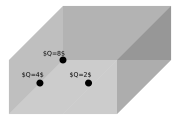
\includegraphics[width=8cm]{Q.png}
\end{center}

\begin{mdframed}[style=MyFrame1]
    \begin{defn}
    \end{defn}
    \cusTitle{Índice de directividad}
    \begin{equation*}
        D_I = 10 \log (Q)
    \end{equation*}
\end{mdframed}


\section{Modelo de esfera pulsante}

Una fuente pulsante monopolar impone una velocidad de partículas en dirección radial, generando un frente de onda esférico.

\begin{mdframed}[style=MyFrame1]
    \begin{defn}
        \label{defn:Q_v}
    \end{defn}
    \cusTitle{Caudal de velocidad particular}
    \begin{equation*}
        Q_v = S\,v(r)
    \end{equation*}
\end{mdframed}

El caudal de velocidad $Q_v$ que produzca una esfera pulsante de radio $a$ es:
\begin{equation*}
    Q_v = 4\pi a^2 \, v(a)
\end{equation*}

Donde $v(r)$ es la velocidad de partículas que impone la esfera pulsante sobre su superficie. Evaluando $r=a$ en la ecuación \ref{eqn:v(r)} podemos escribir el caudal de velocidad como:
\begin{equation*}
    Q_v = 4\pi a^2 \, \frac{A}{\rho_0 \, c} \, \frac{e^{- \iu k a}}{a} \left( 1 - \frac{\iu}{k \, a} \right)
\end{equation*}

Resolviendo para $A$ se tiene:
\begin{align*}
    A &=  \frac{Q_v \, \rho_0 \, c}{4\pi a} \, \frac{e^{\iu k a}}{1 - \frac{\iu}{k \, a}}
    \\
    &= \frac{Q_v \, \rho_0 \, c}{4\pi a} \, \frac{e^{\iu k a}}{\tfrac{\iu k a + 1}{\iu k a}}
    \\
    &= \frac{Q_v \, \rho_0 \, c}{4\pi a} \, \frac{e^{\iu k a}}{\iu k a + 1} \, \frac{\iu \omega a}{c}
    \\
    &= \frac{\iu \omega \, Q_v \, \rho_0 }{4\pi} \, \frac{e^{\iu k a}}{1+\iu ka}
\end{align*}

Reemplazar esta amplitud calculada en la ecuación \ref{eqn:p(r)} permite definir la presión que genera la fuente en función de la distancia $r$ al centro de la esfera.
\begin{equation*}
    p(r) = \frac{\iu \omega \, Q_v \, \rho_0 }{4\pi} \, \frac{1}{1+\iu k a} \, \frac{e^{-\iu k (r-a)}}{r}
\end{equation*}

Considerar como hipótesis que $ka<<1$ supone que la fuente sea puntual, obteniendo para la presión:
\begin{equation}
    p(r) = \frac{\iu \omega \, Q_v \, \rho_0 }{4\pi} \, \frac{e^{-\iu k (r-a)}}{r}
    \label{eqn:p(r)withA}
\end{equation}

A partir de la definición \ref{defn:particlesVelocity}, al derivar la presión obtenida anteriormente, podemos determinar la velocidad de partículas que genera la fuente en función de la distancia $r$ al centro de la esfera.
\begin{align*}
    v(r) &= \frac{\iu}{\rho_0 \, c \, k } \, \frac{\dif p(r)}{\dif r}
    \\
    &= \frac{\iu}{\rho_0 \, c \, k } \, \frac{\iu \omega \, Q_v \, \rho_0 }{4\pi} \, \frac{\dif}{\dif r} \left[ \frac{e^{-\iu k (r-a)}}{r} \right]
    \\
    &= - \frac{Q_v}{4\pi} \, \frac{\dif}{\dif r} \left[ \frac{e^{-\iu k (r-a)}}{r} \right]
    \\
    &= - \frac{Q_v}{4\pi} \left[ -\iu k \frac{e^{-\iu k (r-a)}}{r} - \frac{e^{-\iu k (r-a)}}{r^2} \right]
    \\
    &= \frac{Q_v}{4\pi} \, \frac{e^{-\iu k (r-a)}}{r} \left( \frac{1}{r} + \iu k \right)
\end{align*}

Y su conjugado:
\begin{equation*}
    \overline{v}(r) = \frac{Q_v}{4\pi} \, \frac{e^{\iu k (r-a)}}{r} \left( \frac{1}{r} - \iu k \right)
\end{equation*}

De manera que el producto $p(r)\,\overline{v}(r)$ queda:
\begin{align*}
    p(r)\,\overline{v}(r) &= \frac{\iu \omega \, Q_v \, \rho_0 }{4\pi} \, \frac{e^{-\iu k (r-a)}}{r} \, \frac{Q_v}{4\pi} \, \frac{e^{\iu k (r-a)}}{r} \left( \frac{1}{r} - \iu k \right)
    \\
    &= \left(\frac{Q_v}{4\pi r}\right)^2 \left( \frac{\iu \, \omega \, \rho_0}{r} + \omega \, \rho_0 \, k \right)
    \\
    &= \left(\frac{Q_v}{4\pi r}\right)^2 \left( \frac{\omega^2 \, \rho_0}{c} + \iu \, \frac{\omega \, \rho_0}{r} \right)
\end{align*}

Tomando la parte real del producto anterior se obtiene, a partir de la propiedad \ref{prop:aveI}, la siguiente expresión para la intensidad:
\begin{align*}
    I &= \frac{\Re \left[ p(r)\,\overline{v}(r) \right]}{2}
    \\
    &= \left(\frac{Q_v}{4\pi r}\right)^2 \frac{\omega^2 \, \rho_0}{2c}
\end{align*}

La intensidad fue definida como la potencia por unidad de superficie (Def. \ref{defn:I}) luego $W=I\,S=I\,4\pi r^2$ pudiendo definir la potencia acústica al reemplazar la intensidad según:

\begin{mdframed}[style=MyFrame1]
    \begin{prop}
    \end{prop}
    \cusTitle{Potencia de fuente esférica puntual}
    \begin{equation*}
        W = \frac{Q_v^2 \, \rho_0 \, \omega^2}{8\pi \,c}
    \end{equation*}
\end{mdframed}

Por otro lado, podemos tomar la presión eficaz al cuadrado a partir de la ecuación \ref{eqn:p(r)withA} obteniendo:
\begin{align*}
    \rms{p}^2 &= \frac{\norm{p(r)}^2}{2}
    = \frac{1}{2} \, \norm{\frac{\iu \omega \, Q_v \, \rho_0 }{4\pi} \, \frac{e^{-\iu k (r-a)}}{r}}^2
    \\
    &= \frac{1}{2} \, \left(\frac{\omega \, Q_v \, \rho_0 }{4\pi r}\right)^2
    = \frac{1}{2} \, \frac{Q_v^2 \, \rho_0 \, \omega^2}{4\pi} \, \frac{\rho_0}{4\pi r^2}
    \\
    &= \frac{Q_v^2 \, \rho_0 \, \omega^2}{8\pi \, c} \, \frac{\rho_0 \, c}{4\pi r^2}
\end{align*}

Es necesario agregar como hipótesis que $k\,r>>1$ para considerar que la radiación se da en campo lejano. Así, en la ecuación anterior, la impedancia está dada por $Z=\rho_0 \, c$ en efecto. Luego:

\begin{mdframed}[style=MyFrame1]
    \begin{prop}
        \label{prop:p^2/Z=W/S}
    \end{prop}
    Se tiene una fuente de sonido esférica, cuyo coeficiente de reflexión es $R=0$ y coeficiente de directividad $Q=1$. Sea $k\, a<<1$ pudiendo considerarse la fuente puntual. Sea $k\,r>>1$ pudiendo considerarse la radiación en campo lejano. Entonces se cumple:
    \begin{equation*}
        \frac{\rms{p}^2}{Z\,Q} = \frac{W}{S}
    \end{equation*}
    Donde $S=4\pi r^2$ es la superficie de radiación y $Z=\rho_0 \, c$ la impedancia característica del medio.
\end{mdframed}

Observar que cumplirse simultáneamente $k\, a<<1$ y $k\,r>>1$ implica que $r>>a$ lo cual significa que la propiedad se verifica para todas las frecuecias, por ser independiente de $k$.


\subsection{Ley cuadrática inversa}
\label{sec:inverseSquareLaw}

Haciendo algunos despejes en la propiedad \ref{prop:p^2/Z=W/S} se puede hallar una importante simetría.
\begin{align*}
    \frac{\rms{p}^2}{\rho_0 \, c} &= \frac{W}{4\pi r^2}
    \\
    \norm{\rms{p} \, r} &= \sqrt{\frac{W \, \rho_0 \, c}{4\pi}} = \textrm{constante}
\end{align*}

Lo cual implica:

\begin{mdframed}[style=MyFrame1]
    \begin{prop}
    \end{prop}
    La presión multiplicada por la distancia es constante.
    \begin{equation*}
        \Delta \norm{\rms{p} \, r} = 0
    \end{equation*}
\end{mdframed}

Pudiendo escribir:
\begin{align*}
    {\rms{p}}_1 \, r_1 &= {\rms{p}}_2 \, r_2
    \\
    \frac{{\rms{p}}_1}{{\rms{p}}_2} &= \frac{r_2}{r_1}
    \\
    \frac{\tfrac{{\rms{p}}_1}{\sub{p}{ref}}}{\tfrac{{\rms{p}}_2}{\sub{p}{ref}}} &= \frac{r_2}{r_1}
    \\
    20 \log \left( \frac{{\rms{p}}_1}{\sub{p}{ref}} \right) - 20 \log \left( \frac{{\rms{p}}_2}{\sub{p}{ref}} \right) &= 20 \log \left( \frac{r_2}{r_1} \right)
    \\
    \Delta L_p = 20 \log \left( \frac{r_2}{r_1} \right)
\end{align*}

Luego si la distancia $r_2$ es el doble de $r_1$ queda:
\begin{equation*}
    \Delta L_p = 20 \log \left( \frac{2 \, r_1}{r_1} \right) \approx 6\,\si{\deci\bel}
\end{equation*}


\section{Dipolo acústico} % Falta terminar (ver unidad 4)


\section{Bafle infinito} % Falta terminar (ver unidad 4)


\section{Modelo de Line Array} % Falta terminar (ver unidad 4)

\clearpage % Provisorio
\section{Niveles de presión, intensidad y potencia}

Para estudiar las variaciones de presión, intensidad y potencia, se definen niveles en escalas logarítmicas. Los respectivos niveles relacionan dichas magnitudes con un valor de referencia, indicando qué tan por encima están del umbral de audición.

\begin{mdframed}[style=MyFrame1]
    \begin{defn}
    \end{defn}
    \cusTitle{Presión de referencia}
    \cusText{Mínima presión perceptible por el oído humano.}
    \begin{equation*}
        \sub{p}{ref} = 20\,\si{\micro\pascal}
    \end{equation*}
\end{mdframed}

Reemplazando $\sub{p}{ref}$ en la propiedad \ref{prop:p^2/Z=W/S} se obtiene la intensidad de referencia en el aire para ondas planas en campo lejano:
\begin{equation*}
    \sub{I}{ref}=\frac{(20\,\si{\micro\pascal})^2}{1.18\,\si{\kilo\gram\per\metre^2} \cdot 343\,\si{\metre\per\second}} = 10^{-12}\,\si{\watt\per\metre^2}
\end{equation*}

Reemplazando $\sub{I}{ref}$ en la definición \ref{defn:I} se tiene que la mínima potencia que puede percibir el humano, para una superficie de radiación $S=1\,\si{\metre^2}$, es:
\begin{equation*}
    \sub{W}{ref} = 10^{-12}\,\si{\watt}
\end{equation*}

\begin{mdframed}[style=MyFrame1]
    \begin{defn}
        \label{defn:SPL}
    \end{defn}
    \cusTitle{Nivel de presión sonora}
    \begin{equation*}
        L_p = SPL = 20 \log \left( \frac{\rms{p}}{\sub{p}{ref}} \right) \si{\deci\bel}
    \end{equation*}
\end{mdframed}

\begin{mdframed}[style=MyFrame1]
    \begin{defn}
        \label{defn:SIL}
    \end{defn}
    \cusTitle{Nivel de intensidad sonora}
    \begin{equation*}
        L_I = SIL = 10 \log \left( \frac{I}{\sub{I}{ref}} \right)\si{\deci\bel}
    \end{equation*}
\end{mdframed}

\begin{mdframed}[style=MyFrame1]
    \begin{defn}
        \label{defn:PWL}
    \end{defn}
    \cusTitle{Nivel de potencia acústica}
    \begin{equation*}
        L_W = PWL = 10 \log \left( \frac{W}{\sub{W}{ref}} \right)\si{\deci\bel}
    \end{equation*}
\end{mdframed}

Para ondas planas en campo libre se puede usar la propiedad \ref{prop:p^2/Z=W/S} en la definición \ref{defn:SIL}, quedando:
\begin{equation*}
    SIL = 10 \log \left( \frac{\rms{p}^2}{\rho_0 \, c \, \sub{I}{ref}} \right) \si{\deci\bel}
\end{equation*}

Se multiplica el argumento del logaritmo por $\tfrac{\sub{p}{ref}^2}{\sub{p}{ref}^2}$ sin alterar la igualdad, y luego se reagrupa usando propiedades logarítmicas:
\begin{align*}
    SIL &= 10 \log \left( \frac{\rms{p}^2}{\sub{p}{ref}^2} \frac{\sub{p}{ref}^2}{\rho_0 \, c \, \sub{I}{ref}} \right) \si{\deci\bel}
    \\
    &= 20 \log \left( \frac{\rms{p}}{\sub{p}{ref}} \right) \si{\deci\bel} + 10 \log \left( \frac{\sub{p}{ref}^2}{\rho_0 \, c \, \sub{I}{ref}} \right) \si{\deci\bel}
\end{align*}

Verificándose la siguiente propiedad.

\begin{mdframed}[style=MyFrame1]
    \begin{prop}
    \end{prop}
    Para ondas planas y en campo libre:
    \begin{equation*}
        SIL = SPL + 10 \log \left( \frac{\sub{p}{ref}^2}{\rho_0 \, c \, \sub{I}{ref}} \right) \si{\deci\bel}
    \end{equation*}
\end{mdframed}

En la que el segundo término tiende a anularse si los valores de $\sub{I}{ref}$, $\sub{p}{ref}$, $\rho_0$ y $c$ están dados para condiciones normales de presión y temperatura, quedando:
\begin{equation*}
    SIL \approx SPL
\end{equation*}

Despejando $\rms{p}^2$ de la propiedad \ref{prop:p^2/Z=W/S}, y reemplazando luego este valor en la definición de nivel de presión sonora (Def. \ref{defn:SPL}) se tiene:
\begin{align*}
    L_p &= 10 \log \left( \frac{W \, \rho_0 \, c \, Q}{S \, \sub{p}{ref}^2} \right) \si{\deci\bel}
    \\
    &= \left[ 10\log \left( \frac{\rho_0 \, c}{\sub{p}{ref}^2} \right) + 10\log(W) + 10\log \left( \frac{Q}{S} \right) \right] \si{\deci\bel}
    \\
    &= 120 \si{\deci\bel} + 10 \log(W)\,\si{\deci\bel} + 10 \log \left( \frac{Q}{S} \right) \si{\deci\bel}
\end{align*}

Aplicando la definición de nivel de potencia (Def. \ref{defn:PWL}) al sumando $120\,\si{\deci\bel}$ se tiene:
\begin{align*}
    L_p &= \left[ 10 \log \left( \frac{1}{10^{-12}} \right) + 10 \log(W) + 10 \log \left( \frac{Q}{S} \right) \right] \si{\deci\bel}
    \\
    &= 10 \log \left( \frac{W}{10^{-12}} \right) + 10 \log \left( \frac{Q}{S} \right) \si{\deci\bel}
\end{align*}

Obteniendo la siguiente propiedad.

\begin{mdframed}[style=MyFrame1]
    \begin{prop}
    \end{prop}
    Para ondas planas y en campo libre:
    \begin{equation*}
        L_p = L_W + 10 \log \left( \frac{Q}{S} \right) \si{\deci\bel}
    \end{equation*}
\end{mdframed}

De manera que si la superficie es unitaria $S=1\,\si{\metre^2}$ se tiene que:
\begin{equation*}
    PWL \approx SPL \approx SIL
\end{equation*}


\chapter{Ondas estacionarias}
\label{cha:standingWaves}

Una onda estacionaria es aquella que presenta puntos de amplitud nula que están fijos en el espacio, llamados nodos. Resulta de la interferencia entre dos ondas de igual amplitud, longitud de onda y frecuencia pero que avanzan en sentido opuesto.

En la naturaleza este fenómeno puede darse, por ejemplo, en sogas para ondas transversales o en tubos para ondas longitudinales. En estos casos, el modelo matemático usado es el de onda de una dimensión válido para frecuencias menores a:
\begin{equation*}
    f_c = \frac{1.84 \, c}{2\pi r}
\end{equation*}

Ya que para frecuencias mayores o para tubos de un radio $r>>\lambda$ pueden formarse ondas estacionarias transversales. El comportamiento \emph{modal} de conductos de mayor radio o de recintos en general se analiza a partir de ondas tridimensionales.


\section{Resonancia en tubos}

Se dice que un tubo está en resonancia cuando uno de sus dos extremos está siendo excitado periódicamente por una perturbación de manera que se formen ondas estacionarias en el interior.

El extremo donde se da la perturbación periódica se modela mediante un pistón rígido que se mueve a una frecuencia angular $\omega$ hacia adelante y hacia atrás. El otro extremo o bien puede estar abierto o bien puede ser cerrado por una tapa rígida. En ambos casos, se genera una onda reflejada debido al cambio de impedancia. Con lo cual, las funciones de presión y velocidad están dadas por las ecuaciones \ref{eqn:Helmholtz} y \ref{eqn:particleVel1D} respectivamente:
\begin{gather}
    p(x) = A \, e^{-\iu k x} + B \, e^{\iu k x}
    \label{eqn:tubePressure}
    \\
    v(x) = \frac{A}{\rho_0 \, c} \, e^{-\iu k x} - \frac{B}{\rho_0 \, c} \, e^{\iu k x}
    \label{eqn:tubeVelocity}
\end{gather}

De todas las frecuencias que pueda generar el pistón, solo van a ser resonantes aquellas para las que el tiempo en que tarde el pistón en realizar un ciclo esté sincronizado con el tiempo que tarda la onda en recorrer el tubo ida y vuelta. De esta forma, la onda reincide en el pistón cuando este está en la posición de equilibrio generando un nuevo frente de onda coincidente con el anterior. En este extremo, la velocidad de las partículas va a ser determinada por la frecuencia impuesta por el pistón.
\begin{equation}
    v(x_0) = v_\omega
    \label{eqn:tubeV0}
\end{equation}

Consideremos el caso en que el otro extremo está cerrado por una tapa rígida, como se muestra en el esquema a continuación.

\begin{center}
    \includegraphics[width=5.7cm]{tubeCC.png}
\end{center}

Dado que las partículas no van a poder moverse más allá de la tapa, la velocidad particular en ese punto será nula. Por lo tanto, podemos asumir como hipótesis que en $x=L$ la impedancia es infinita.
\begin{equation*}
    \left\{
    \begin{aligned}
        p(L) &\to \infty
        \\
        v(L) &\to 0
    \end{aligned}
    \right.
    \implies
    Z \to \infty
\end{equation*}

A partir de estas hipótesis, evaluando $x=L$ en la ecuación \ref{eqn:tubeVelocity} y considerando la ecuación \ref{eqn:tubeV0} para $x=0$, se tiene que para cada extremo la velocidad de partículas es:
\begin{equation*}
    \left\{
    \begin{aligned}
        v(L) &= 0 = \frac{A}{\rho_0 \, c} e^{-\iu k L} - \frac{B}{\rho_0 \, c} e^{\iu k L}
        \\
        v(x_0) &= v_\omega = \frac{A}{\rho_0 \, c} - \frac{B}{\rho_0 \, c}
    \end{aligned}
    \right.
\end{equation*}

De este sistema se despeja $A = B \, e^{2 \iu kL}$ de la primer ecuación y se reemplaza en la segunda para obtener:
\begin{equation*}
    v_\omega \, \rho_0 \, c = B \, e^{2 \iu kL} - B
\end{equation*}

Y al despejar $B$:
\begin{align*}
    B &= \frac{v_\omega \, \rho_0 \, c}{e^{2 \iu kL}-1}
    \\
    &= \frac{v_\omega \, \rho_0 \, c \, e^{-\iu kL}}{e^{\iu kL}-e^{-\iu kL}}
    \\
    &= \frac{v_\omega \, \rho_0 \, c}{2\iu \sin(kL)} \, e^{-\iu kL}
\end{align*}

Se resuelve para $A$:
\begin{equation*}
    A = \frac{v_\omega \, \rho_0 \, c}{2\iu \sin(kL)} \, e^{\iu kL}
\end{equation*}

A partir de los coeficientes $A$ y $B$ calculados, la ecuación \ref{eqn:tubeVelocity} queda dada por:
\begin{align*}
    v(x) &=
    \frac{v_\omega}{2\iu \sin(kL)} \, e^{\iu k(L-x)}
    - \frac{v_\omega}{2\iu \sin(kL)} \, e^{\iu k(x-L)}
    \\
    &= \frac{v_\omega}{2\iu \sin(kL)} \Big[ e^{\iu k(L-x)} - e^{-\iu k(L-x)} \Big]
    \\
    &= v_\omega \, \frac{\sin(kL-kx)}{\sin(kL)}
\end{align*}

A partir de la velocidad, podemos encontrar la presión según la definición \ref{defn:particlesVelocity} integrándo la velocidad:
\begin{align*}
    p(x) &= \frac{\rho_0 \, c \, k}{\iu} \int v(x) \, \dif x
    \\
    &= \frac{\rho_0 \, c \, k}{\iu} \int v_\omega \, \frac{\sin(kL-kx)}{\sin(kL)} \, \dif x
    \\
    &= \frac{\rho_0 \, c \, k \, v_\omega}{\iu \sin(kL)} \, \int \sin(kL-kx) \, \dif x
    \\
    &= \rho_0 \, c \, v_\omega \, \frac{\cos (kL-kx)}{\iu \sin(kL)}
\end{align*}

De manera que la impedancia (Def. \ref{defn:impedance}) a lo largo del tubo está determinada por:
\begin{equation}
    Z(x) = \frac{\rho_0 \, c}{\iu \tan(kL-kx)}
\end{equation}

Por lo tanto, las frecuencias de resonancia van a ser aquellas que verifiquen que $Z(x)$ evaluado en $x_0=0$ tiende a infinito:
\begin{gather*}
    Z(x_0) \to \infty
    \iff
    \tan(kL-kx_0) \to 0
    \\
    \therefore
    k\,L = n\,\pi
\end{gather*}

O bien escribiendo $k=2\pi\, f/c$ se tiene que las frecuencias de resonancias son:
\begin{equation}
    f = \frac{n \, c}{2 \, L}
\end{equation}

O bien escribiendo $k=2\pi/\lambda$ se tiene que las longitudes de onda que pongan el tubo en resonancia son:
\begin{equation}
    \lambda = \frac{2 \, L}{n}
\end{equation}

Consideremos el caso en que el otro extremo está abierto, como se muestra en el esquema a continuación

\begin{center}
    \includegraphics[width=5.7cm]{tubeCO.png}
\end{center}

En el extremo abierto las partículas pueden moverse libremente con velocidad particular máxima, dándose un punto de presión mínima. Por lo tanto, podemos asumir como hipótesis que en $x=L$ la impedancia va a ser nula.
\begin{equation*}
    \left\{
    \begin{aligned}
        p(L) &\to 0
        \\
        v(L) &\to \infty
    \end{aligned}
    \right.
    \implies
    Z \to 0
\end{equation*}

Pudiendo demostrar con un desarrollo similar al caso anterior que la impedancia está dada por:
\begin{equation}
    Z(x) = \iu \, \rho_0 \, c \tan (kL-kx)
\end{equation}

Y las frecuencias de resonancia:
\begin{equation}
    f = \frac{\left( 2n+1 \right) c}{4 \, L}
\end{equation}

Con armónicos impares de longitud de onda:
\begin{equation}
    \lambda = \frac{4 \, L}{2n + 1}
\end{equation}


\section{Modos}

Se define la frecuencia de Schroeder que determina empíricamente a partir de qué frecuencia el análisis modal de un recinto no puede aplicarse para determinar la deformada modal.

\begin{mdframed}[style=MyFrame1]
    \begin{defn}
    \end{defn}
    \cusTitle{Frecuencia de Schroeder}
    \begin{equation*}
        f_S = 2000 \sqrt{\frac{\sub{TR}{mid}}{V}}
    \end{equation*}
\end{mdframed}

Donde $\sub{TR}{mid}$ es el tiempo de reverberación medio definido como:
\begin{equation*}
    \sub{TR}{mid} = \frac{TR(500\,\si{\hertz})+TR(1\,\si{\kilo\hertz})}{2}
\end{equation*}

Partiendo de la ecuación de Helmholtz (Def. \ref{defn:Helmholtz3D}) en 3 dimensiones para coordenadas cartesianas:
\begin{equation*}
    \grad^2 p(\Vec{x}) + k^2 \, p(\Vec{x}) = 0
\end{equation*}

Podemos disociar las variables:
\begin{equation*}
    \grad^2 \left[ p_x(x) \, p_y(y) \, p_z(z) \right] + k^2 \, p_x(x) \, p_y(y) \, p_z(z) = 0
\end{equation*}

Y al dividir por $p_x(x) \, p_y(y) \, p_z(z)$ se obtiene:
\begin{equation*}
    \frac{\grad^2 \left[ p_x(x) \, p_y(y) \, p_z(z) \right]}{p_x(x) \, p_y(y) \, p_z(z)} + k^2 = 0
\end{equation*}

Al aplicar el laplaciano, las funciones que no dependan de la variable independiente que se derive permanecen constantes:
\begin{equation}
    \frac{1}{p_x(x)} \, \frac{\partial^2 p(x)}{\partial x^2}
    + \frac{1}{p_y(y)} \, \frac{\partial^2 p(y)}{\partial y^2}
    + \frac{1}{p_z(z)} \, \frac{\partial^2 p(z)}{\partial z^2}
    + k^2 = 0
    \label{eqn:modesHelmholtz}
\end{equation}

Se define el número de onda como:
\begin{equation}
    k^2 = k_x^2 + k_y^2 + k_z^2
    \label{eqn:modesk^2}
\end{equation}

De modo que la ecuación \ref{eqn:modesHelmholtz} sea implicada por la suma de las tres ecuaciones del siguiente sistema.
\begin{gather*}
    \impliedby
    \left\{
    \begin{aligned}
        \frac{1}{p_x(x)} \, \frac{\partial^2 p(x)}{\partial x^2} + k_x^2 = 0
        \\
        \frac{1}{p_y(y)} \, \frac{\partial^2 p(y)}{\partial y^2} + k_y^2 = 0
        \\
        \frac{1}{p_z(z)} \, \frac{\partial^2 p(z)}{\partial z^2} + k_z^2 = 0
    \end{aligned}
    \right.
    \\
    \iff
    \left\{
    \begin{aligned}
        \frac{\partial^2 p(x)}{\partial x^2} + k_x^2 \, p_x(x) = 0
        \\
        \frac{\partial^2 p(y)}{\partial y^2} + k_y^2 \, p_y(y) = 0
        \\
        \frac{\partial^2 p(z)}{\partial z^2} + k_z^2 \, p_z(z) = 0
    \end{aligned}
    \right.
\end{gather*}

Siendo cada solución $p_x(x)$, $p_y(x)$ y $p_z(x)$ del tipo $p_x(x) = C_x \cos (k_x x + \varphi)$ luego la velocidad de partículas está dada análogamente según la definición \ref{defn:particlesVelocity} por:
\begin{equation*}
    v_x(x) = \frac{\iu}{\rho_0 \, c \, k_x} \, \frac{\partial p_x(x)}{\partial x} = - \frac{\iu \, C_x}{\rho_0 \, c} \sin (k_x x + \varphi)
\end{equation*}

Por hipótesis de contorno, se tiene que cumplir para $x_0=0$ que $v(x_0) = 0$ y $v(L_x) = 0$ simultáneamente.
\begin{gather*}
    v(x_0) = - \frac{\iu \, C_x}{\rho_0 \, c} \sin (\varphi) = 0
    \\
    \implies \varphi = 0
    \\
    \therefore \, v(L_x) = - \frac{\iu \, C_x}{\rho_0 \, c} \sin (k_x L_x) = 0
    \\
    \implies k_x L_x = n_x \pi \implies k_x = \frac{n_x \pi}{L_x}
\end{gather*}

Reemplazando $k_x$, y luego con el mismo razonamiento $k_y$ y $k_z$, en la ecuación \ref{eqn:modesk^2} queda definida la frecuencia de resonancia propia del recinto.
\begin{gather*}
    k^2 = \left( \frac{\omega}{c} \right)^2 =
    \\
    \left( \frac{2\pi\,f_0}{c} \right)^2
    = \left( \frac{n_x \, \pi}{L_x} \right)^2 + \left( \frac{n_y \, \pi}{L_y} \right)^2 + \left( \frac{n_z \, \pi}{L_z} \right)^2
\end{gather*}

\begin{mdframed}[style=MyFrame1]
    \begin{defn}
    \end{defn}
    \cusTitle{Frecuencias modales}
    \cusText{Frecuencias de resonancia que excitan los modos propios de un recinto rectangular.}
    \begin{equation*}
        f_0 = \frac{c}{2} \sqrt{\left(\frac{n_x}{L_x}\right)^2 + \left(\frac{n_y}{L_y}\right)^2 + \left(\frac{n_z}{L_z}\right)^2}
    \end{equation*}
\end{mdframed}


\section{Criterios empíricos}


\subsection{Criterio de Bolt}

Richard H. Bolt propone en 1946 que los recintos de óptima escucha serán los que tengan una distribución frecuencial homogénea entre modos. El criterio de Bolt se verifica para salas con dimensiones proporcionales a las siguientes siendo $L_z$ unitario:

\begin{equation*}
    \left\{
    \begin{aligned}
        & \frac{3}{2} \left( L_x-1 \right) < L_y -1 < 3 \left( L_x-1 \right)
        \\
        & 2 < L_x+L_y < 4
    \end{aligned}
    \right.
\end{equation*}


\subsection{Criterio de Bonello}

Oscar J. Bonello determina en 1981 un criterio para la mejor distribución de los modos normales de una sala a partir de la \emph{densidad modal} o cantidad de modos por debajo de cierta frecuencia.
\begin{equation*}
    N(f) = \frac{4\pi\,V}{3} \left(\frac{f}{c}\right)^3 + \frac{\pi \, S}{4} \left(\frac{f}{c}\right)^2 + \frac{L}{8} \left(\frac{f}{c}\right)
\end{equation*}

De manera que una sala será libre de coloración si:
\begin{itemize}
    \item La cantidad de modos en función de la frecuencia es monótonamente creciente.
    \item No tiene modos dobles para bandas con menos de 5 modos
\end{itemize} 


\subsection{Criterio de Cox}

Trevor J. Cox y Peter D'Antonio establecen en 2001 un método para determinar las dimensiones óptimas de una sala para la escucha crítica. Estudiando la función de transferencia entre sus esquinas, adecuaron las dimensiones para que esta sea lo más plana posible.


\chapter{Acústica geométrica}

Como contrapartida al estudio ondulatorio del sonido, se propone describir la propagación sonora como si de \emph{rayos} se tratase.

Un \emph{rayo de sonido} es una trayectoria rectilínea que acompaña de manera perpendicular el frente de onda. La característica principal que se usa en este enfoque es la reflexión especular. Esto es, si un rayo impacta contra una superficie con cierto ángulo, este se va a reflejar con el mismo ángulo. Pero cabe destacar que los rayos de sonido no existen como tales en la naturaleza, sino que son un modelo para describir el fenómeno sonoro.

Este enfoque es aplicable para frecuencias altas, para las que se puede despreciar los fenómenos de interferencia y de difracción, y a una distancia tal que el frente de onda pueda considerarse plano.


\section{Suma de presiones}

Consideremos dos o más fuentes de sonido radiando energía de forma esférica en campo libre. Se quiere calcular la presión resultante debida al aporte de todas las fuentes en un punto. Sumar presiones implica sumar las respectivas funciones que describan cómo varía la presión de cada fuente en dicho punto:
\begin{equation*}
    p(\Vec{x}_0,t) = \norm{p} e^{\iu(\omega t + \varphi)}
\end{equation*}

Podría tratarse de señales desfasadas:

\begin{mdframed}[style=MyFrame1]
    \begin{defn}
    \end{defn}
    \cusTitle{Fase}
    \begin{equation*}
        \Delta \varphi = \frac{2\pi}{\lambda} \Delta x = \frac{2\pi}{T} \Delta t
    \end{equation*}
\end{mdframed}

Debido a este comportamiento periódico, pueden darse sumas de presiones que culminen en cancelaciones o amplificaciones. Se definen dos tipos de señales.

\begin{mdframed}[style=MyFrame1]
    \begin{defn}
    \end{defn}
    \cusTitle{Señales correlacionadas}
    \cusText{Son aquellas señales de igual frecuencia.}
    \begin{equation*}
        \omega_1=\omega_2
    \end{equation*}
\end{mdframed}

\begin{mdframed}[style=MyFrame1]
    \begin{defn}
    \end{defn}
    \cusTitle{Señales coherentes}
    \cusText{Son aquellas señales correlacionadas sin desfasaje.}
    \begin{equation*}
        \omega_1=\omega_2 \quad \land \quad \varphi_1=\varphi_2
    \end{equation*}
\end{mdframed}

Planteemos entonces la situación general en la que se quieren sumar dos presiones en un punto a cierta distancia de cada fuente.

Se quiere calcular un valor de presión total que sea representativo de la interacción de ambas señales. Dado que se están sumando funciones periódicas cuyo promedio es nulo, se realiza una \emph{suma energética} elevando al cuadrado el módulo de la presión total.
\begin{align*}
    p_T &= p_1 + p_2
    \\
    \norm{p_T} &= \norm{p_1 + p_2}
    \\
    \norm{p_T}^2 &= \norm{p_1 + p_2}^2
\end{align*}

Para sortear la dependencia temporal y espacial, se usa una propiedad de los números complejos \cite{2} (Pág. 25) que demuestra que:
\begin{equation}
    \norm{p_T}^2 = \norm{p_1}^2 + \norm{p_2}^2 + 2 \norm{p_1}^2 \norm{p_2}^2 \cos(\Delta \theta)
    \label{eqn:|P_T|^2}
\end{equation}

Donde $\cos(\Delta \theta)$ es el factor de correlación dado por:
\begin{equation*}
    \Delta \theta = \left( \omega_1 t + \varphi_1 \right) - \left( \omega_2 t + \varphi_2 \right) = \Delta \omega \, t + \Delta \varphi
\end{equation*}


\subsection{Suma correlacionada}

Consideremos dos señales correlacionadas que, por definición, tienen la misma frecuencia. Reemplazando $\omega_1=\omega_2$ en la ecuación \ref{eqn:|P_T|^2} la suma queda dada por:
\begin{equation*}
    \norm{p_T}^2 = \norm{p_1}^2 + \norm{p_2}^2 + 2 \norm{p_1}^2 \norm{p_2}^2 \cos(\Delta \varphi)
\end{equation*}

Podemos suponer que las presiones que están siendo sumadas tienen la misma amplitud.
\begin{equation*}
    \norm{p_1} = \norm{p_2} = \rms{p}
\end{equation*}

De esta forma se analizaría la variación del nivel de presión sonora al duplicar la presión eficaz, en función de la diferencia de fase entre ambas presiones. Identificamos así tres situaciones destacables.

\begin{itemize}
    \item \cusTitle{Suma completa:}
    $\Delta \varphi = \ang{0} \implies \cos(\Delta \varphi)=1$
    \begin{align*}
        \norm{p_T}^2 &= \norm{p_1}^2 + \norm{p_2}^2 + 2\norm{p_1} \norm{p_2}
        \\
        &= ( \norm{p_1} + \norm{p_2} )^2
        \\
        &= (2\,\rms{p})^2
        \\
        SPL_T &= 10 \log \left[ \frac{(2\,\rms{p})^2}{\sub{p}{ref}^2} \right] \si{\deci\bel}
        \\
        &= 20 \log \left( 2 \right) \si{\deci\bel} + 20 \log \left( \frac{\rms{p}}{\sub{p}{ref}} \right) \si{\deci\bel}
        \\
        &= 6\,\si{\deci\bel} + SPL
    \end{align*}
    
    \item \cusTitle{Suma parcial:}
    $\Delta \varphi = \ang{90} \implies \cos(\Delta \varphi)=0$
    \begin{align*}
        \norm{p_T}^2 &= \norm{p_1}^2 + \norm{p_2}^2 = 2\,\rms{p}^2
        \\
        SPL_T &= 10 \log \left( \frac{2\,\rms{p}^2}{\sub{p}{ref}^2} \right) \si{\deci\bel}
        \\
        &= 10 \log \left( 2 \right) \si{\deci\bel} + 20 \log \left( \frac{\rms{p}}{\sub{p}{ref}} \right) \si{\deci\bel}
        \\
        &= 3\,\si{\deci\bel} + SPL
    \end{align*}
    
    \item \cusTitle{Cancelación:}
    $\Delta \varphi = \ang{180} \implies \cos(\Delta \varphi)=-1$
    \begin{align*}
        \norm{p_T}^2 &= \norm{p_1}^2 + \norm{p_2}^2 - 2\norm{p_1} \norm{p_2}
        \\
        &= ( \norm{p_1} - \norm{p_2} )^2 = 0
        \\
        SPL_T &= 10 \log \left( \frac{0}{\sub{p}{ref}^2} \right) \si{\deci\bel}
        = -\infty\,\si{\deci\bel}
\end{align*}
\end{itemize}

A partir de estas situaciones particulares, se puede inferir el comportamiento general de la presión sumada en función de la fase.

A continuación se muestra, para un desfasaje de $\ang{0}$ a $\ang{360}$, valores de grises que representan la cancelación (en negro) o amplificación (en blanco) que resulta de sumar dos presiones de igual magnitud.

\begin{center}
    \includegraphics[width=3.8cm]{phaseSum.png}
\end{center}


\subsection{Suma no correlacionada}

La suma de señales que tengan diferentes frecuencias puede ser hecha según la ecuación \ref{eqn:|P_T|^2} misma.

Pero en este caso, dado que $\omega_1\neq\omega_2$, el factor de correlatividad $\cos(\Delta \omega \, t + \Delta \varphi)$ va a estar en función del tiempo. Esto implica que la suma de las presiones va a producir cancelaciones y amplificaciones de manera periódica. Como está acotado entre $+1$ y $-1$, el factor de correlatividad tomará ese rango de valores conforme transcurra el tiempo. Por lo tanto, a veces la suma va a producir una presión de $+6\,\si{\deci\bel}$ y a veces una cancelación de $-\infty\,\si{\deci\bel}$, como máximo si las presiones son de igual módulo.

Por este motivo no es posible determinar casos particulares para distintos valores de desfasaje. En contrapartida, se puede determinar un valor que represente la presión total promedio que esté siendo sumada.
\begin{align*}
    \rms{\norm{p_T}} &= \sqrt{\frac{1}{2\pi} \int_0^{2\pi} \norm{p_T}^2 \dif t}
    \\
    &= \scale{0.8}{\sqrt{\frac{1}{2\pi} \int_0^{2\pi} \left[ \norm{p_1}^2 + \norm{p_2}^2 + 2 \norm{p_1}^2 \norm{p_2}^2 \cos( \Delta \omega \, t + \Delta \varphi) \right] \dif t}}
    \\
    &= \sqrt{\norm{p_1}^2 + \norm{p_2}^2}
\end{align*}

Elevando al cuadrado y dividiendo por $\sub{p}{ref}^2$ en la ecuación anterior queda la suma energética:
\begin{equation*}
    \frac{\rms{{p_T}^2}}{\sub{p}{ref}^2} = \frac{\norm{p_1}^2+\norm{p_2}^2}{\sub{p}{ref}^2} = \sum_{\ith=1}^\nth \frac{\norm{p_\ith}^2}{\sub{p}{ref}^2}
\end{equation*}

El nivel de presión total en decibeles queda dado según la definición \ref{defn:SPL} aplicada a la presión total.

% ¿Cómo es que cada presión |p_n| pico pasa a ser eficaz en la definición?

\begin{mdframed}[style=MyFrame1]
    \begin{defn}
    \end{defn}
    \cusTitle{Nivel de presión global}
    \begin{equation*}
        SPL_T = 10 \log \left( \sum_{\ith=1}^\nth \frac{\rms{p}_\ith^2}{\sub{p}{ref}^2} \right) \si{\deci\bel}
    \end{equation*}
\end{mdframed}

Según la definición \ref{defn:SPL}, cada presión individual es:
\begin{gather*}
    SPL_\ith = 10 \log \left( \frac{\rms{p}_\ith^2}{\sub{p}{ref}^2} \right) \si{\deci\bel}
    \\
    10^{\tfrac{SPL_\ith}{10}} = \frac{\rms{p}_\ith^2}{\sub{p}{ref}^2}
\end{gather*}

Pudiendo reemplazar la sumatoria anterior, obteniendo la siguiente definición equivalente.

\begin{mdframed}[style=MyFrame1]
    \begin{defn}
    \end{defn}
    \cusTitle{Nivel de presión global}
    \begin{equation*}
        SPL_T = 10 \log \left( \sum_{\ith=1}^\nth 10^{\tfrac{SPL_\ith}{10}} \right) \si{\deci\bel}
    \end{equation*}
\end{mdframed}

Por otro lado, el promedio energético se puede calcular a partir de niveles de presión discretos de la siguiente manera.

\begin{mdframed}[style=MyFrame1]
    \begin{defn}
    \end{defn}
    \cusTitle{Nivel de presión promedio}
    \begin{equation*}
        \ave{SPL}=20\log\left(\frac{\sum_{\ith=1}^\nth 10^{\tfrac{L_\ith}{20}}}{N}\right) \si{\deci\bel}
    \end{equation*}
\end{mdframed}


\section{Efecto Doppler}

El efecto Doppler es la variación en la frecuencia relativa de una onda que se debe al movimiento de la fuente respecto del receptor o viceversa.

En el siguiente esquema se tiene una fuente $F$ que emite un sonido de frecuencia $f$ y se mueve en línea recta a velocidad constante $v_F$ hacia un receptor $R$ que está en reposo.

\begin{center}
    \includegraphics[width=7.5cm]{Doppler.png}
\end{center}

Sean
\begin{itemize}
    \item $t_1$ el momento en que la fuente pasa por $x=F_1$.
    \item $t_2$ el momento en que la fuente pasa por $x=F_2$.
    \item $t'_1$ el momento en que la onda emitida en $F_1$ llega a $x=R$.
    \item $t'_2$ el momento en que la onda emitida en $F_2$ llega a $x=R$.
\end{itemize}

Supongamos que la fuente se mueve en silencio hasta que pasa por $F_1$ donde emite sonido. Luego permanece en silencio nuevamente hasta que, transcurrido un intervalo de tiempo equivalente al período $T$ de la onda emitida, emite nuevamente la misma señal.
\begin{equation*}
    t_2-t_1 = T = \frac{D_F}{v_F}
\end{equation*}

Según la velocidad de propagación ($c$) se definen los intervalos de tiempo que tarda en llegar el sonido desde los respectivos puntos de emisión $F_1$ y $F_2$ al receptor $R$.
\begin{gather*}
    \Delta t_1 = t_1' - t_1 = \frac{D_{R1}}{c}
    \\
    \Delta t_2 = t_2' - t_2 = \frac{D_{R2}}{c}
\end{gather*}

El período relativo $T'$ de la onda que escuchará el receptor está dado por:
\begin{equation*}
    T' = t_2'-t_1'
\end{equation*}

Por lo tanto, la frecuencia relativa es:
\begin{align*}
    f' &= \frac{1}{T'}
    \\
    &= \frac{1}{\left( \dfrac{D_{R2}}{c}+t_2 \right) - \left( \dfrac{D_{R1}}{c}+t_1 \right)}
    \\
    &= \frac{1}{\dfrac{D_{R2}}{c} - \dfrac{D_{R1}}{c} + T}
    \\
    &= \frac{1}{\dfrac{-D_F}{c} + T}
    \\
    &= \frac{1}{\dfrac{-T \, v_F}{c} + T}
    \\
    &= \frac{1}{T\left(1-\dfrac{v_F}{c}\right)}
\end{align*}

Siendo la frecuencia relativa escuchada por el receptor mayor a la frecuencia emitida:
\begin{equation*}
    f' = \frac{f}{1-\dfrac{v_F}{c}} > f
\end{equation*}

Lo cual implica que el sonido percibido por el receptor es más agudo que el emitido. Si la fuente estuviese moviéndose en sentido contrario, el signo de $v_F$ sería negativo y la frecuencia relativa sería menor a la frecuencia emitida. Por lo tanto, si la fuente se aleja del receptor, este escucharía un sonido más grave que el emitido.

Esto significa que si la velocidad de la fuente es muy baja comparado con la velocidad de propagación del sonido, la variación en la frecuencia relativa podría ser despreciable. Por otro lado, si la fuente viaja a la velocidad del sonido se genera un frente de onda que por un instante impacta al receptor y luego este percibe la fuente alejándose con una frecuencia relativa más grave.

\begin{mdframed}[style=MyFrame1]
    \begin{defn}
    \end{defn}
    \cusTitle{Número de Match}
    \cusText{El número de Match es una medida de velocidad relativa que se define como el cociente entre la velocidad de un objeto y la velocidad del sonido en el medio en que se mueve dicho objeto.}
    \begin{equation*}
        \mathcal{M} = \frac{v_F}{c}
    \end{equation*}
\end{mdframed}

El siguiente gráfico representa el frente de onda de ona fuente subsónica, de Match 1 y supersónica respectivamente.
\begin{center}
    \includegraphics[width=8cm]{Match.png}
\end{center}

\section{Energía reflejada, absorbida y transmitida}
\label{sec:energyRAT}

Cuando un sonido propagándose se encuentra con un obstáculo, parte del mismo va a ser reflejado, parte absorbido y parte transmitido a través del obstáculo.

\begin{center}
    \includegraphics[width=5cm]{inRAT.png}
\end{center}

Resulta útil estudiar la situación a partir de consideraciones energéticas. La energía incidente será igual a la reflejada, más la absorbida, más la transmitida:
\begin{gather*}
    \sub{E}{in} = E_R + E_A + E_T
    \\
    \frac{\dif \sub{E}{in}}{\dif t} = \sub{W}{in} = W_R + W_A + W_T
    \\
    1 = \frac{W_R}{\sub{W}{in}} + \frac{W_A}{\sub{W}{in}} + \frac{W_T}{\sub{W}{in}}
\end{gather*}

De esta forma, podemos definir coeficientes de reflexión, absorción y transmisión. Estos serán inherentes a las cualidades constructivas del obstáculo.

\begin{mdframed}[style=MyFrame1]
    \begin{defn}
        \label{defn:coefficients}
    \end{defn}
    \cusTitle{Coeficientes energéticos}
    \cusText{Coeficiente de reflexión}
    \begin{equation*}
        \alpha_R = \frac{W_R}{\sub{W}{in}}
    \end{equation*}
    Coeficiente de absorción
    \begin{equation*}
        \alpha = \frac{W_A}{\sub{W}{in}}
    \end{equation*}
    Coeficiente de transmisión
    \begin{equation*}
        \tau = \frac{W_T}{\sub{W}{in}}
    \end{equation*}
\end{mdframed}

Que verifican la siguiente relación:
\begin{equation}
    1 = \alpha_R + \alpha + \tau
    \label{eqn:coefficients}
\end{equation}

Se pueden plantear dos tipos de análisis. Por un lado, se puede estudiar la absorción considerando la hipótesis $\tau=0$ en la ecuación \ref{eqn:coefficients}. Este es el caso de varias aplicaciones de la acústica arquitectónica para el estudio de las reflexiones en recintos. Por otro lado, se puede estudiar la transmisión considerando la hipótesis $\alpha=0$ en la ecuación \ref{eqn:coefficients}. Este es el caso de estudio, por ejemplo, de los silenciadores.


\section{Reflexiones}

Para estudiar las reflexiones de un recinto cerrado o un obstáculo y cómo estas serán percibidas desde cierto punto de escucha, se definen los siguientes conceptos.

\begin{itemize}
    \item \cusTitle{Campo libre}
    \cusText{Espacio de propagación libre de obstáculos y por tanto sin reflexiones.}
    
    \item \cusTitle{Campo cercano}
    \cusText{Espacio donde la impedancia es compleja.}
    
    \item \cusTitle{Campo lejano}
    \cusText{Espacio donde la impedancia imaginaria es despreciable.}
    
    \item \cusTitle{Campo directo}
    \cusText{Espacio no alterado por reflexiones durante el régimen permanente. El nivel de presión cumple la ley cuadrática inversa (Sec. \ref{sec:inverseSquareLaw}).}
    
    \item \cusTitle{Campo difuso o reverberante}
    \cusText{Predominancia de sonido reflejado con igual probabilidad en todas las direcciones durante el régimen permanente. El nivel de presión no disminuye por divergencia, sino que permanece constante al aumentar distancia.}
\end{itemize}

Que pueden ser visualizados en el siguiente gráfico que determina el nivel de presión $SPL$ percibido en función de la distancia $r$ a la fuente.

\begin{center}
    \includegraphics[width=8.5cm]{soundFields.png}
\end{center}

Donde $d_c$ es la distancia crítica y $\mathcal{R}$ la constante de sala, que a su vez depende del coeficiente de absorción promedio $\overline{\alpha}$ definidos a continuación.

\begin{mdframed}[style=MyFrame1]
    \begin{defn}
    \end{defn}
    \cusTitle{Distancia crítica}
    \cusText{Distancia a la que el nivel de presión del campo reverberado es igual al del campo directo.}
    \begin{equation*}
        d_c = \sqrt{\frac{Q\,\mathcal{R}}{16\pi}}
    \end{equation*}
\end{mdframed}

La distancia crítica determina qué tan lejos de la fuente hay que estar para que el sonido directo tenga el mismo nivel que el sonido reverberado.

Esto equivale a considerar $p_T^2=0$ en la ecuación \ref{eqn:criticalDist}, pudiendo despejar $S=4\pi d_c^2$ para inferir la definición anterior.

\begin{mdframed}[style=MyFrame1]
    \begin{defn}
    \end{defn}
    \cusTitle{Constante de sala}
    \begin{equation*}
        \mathcal{R} = \frac{\overline{\alpha} \, S_T}{1-\overline{\alpha}}
    \end{equation*}
\end{mdframed}

\begin{mdframed}[style=MyFrame1]
    \begin{defn}
    \end{defn}
    \cusTitle{Coeficiente de absorción promedio}
    \begin{equation*}
        \overline{\alpha} = \frac{\sum \alpha_\ith \, S_\ith}{S_T}
    \end{equation*}
\end{mdframed}

Consideremos un punto de escucha para una sala en la que una fuente comienza a radiar energía sonora. Al prenderse la fuente, el sonido emitido chocará contra las paredes, el techo y el piso y rápidamente comenzarán a darse reflexiones dentro de la sala. Se estudia, a partir de ese momento, la evolución de la energía aportada por el campo difuso conforme pasa el tiempo.

\begin{itemize}
    \item \cusTitle{Etapa de crecimiento:}
    A medida que el punto es afectado por las reflexiones, la presión aumenta, y por ende la energía también lo hace. Aunque, una porción de la energía es absorbida por las superficies en cada reflexión.
    
    \item \cusTitle{Régimen permanente:}
    A mayor tiempo, las reflexiones que impacten el punto de escucha serán de mayor orden, aportando menos energía. Pero como la fuente sigue radiando, la energía absorbida por la sala cada vez crece más. Para el momento en que la energía absorbida iguale la energía reflejada, la energía en el punto de escucha permanecerá constante.
    
    \item \cusTitle{Etapa de decaimiento:}
    Si la fuente deja de emitir sonido, ya no se generarán nuevas reflexiones. La energía que reciba el punto solo será de las reflexiones ya existentes, hasta que se disipen por completo.
\end{itemize}

A continuación se esquematiza la evolución de la energía de la sala en función del tiempo, descripta anteriormente.

\begin{center}
    \includegraphics[width=4.7cm]{roomEnergy.png}
\end{center}

Se pretende estudiar el aporte energético del capo difuso durante el régimen permanente para cualquier punto de un recinto, independientemente del sonido directo que reciba.

Para esto, se suman los infinitos vectores intensidad de las reflexiones de orden superior que eventualmente van a incidir sobre un elemento de superficie del recinto. Todas las direcciones de incidencia son equiprobables, por estar bajo la hipótesis de campo difuso. La superficie de incidencia es representada en la siguiente figura como la intersección entre un plano vertical y una semiesfera.

\begin{center}
    \includegraphics[width=4.5cm]{diffuseIntegration.png}
\end{center}

El plano vertical corresponde al segmento de superficie sobre la que se quiere evaluar la incidencia. Los versores normales de la superficie semiesférica representan las direcciones de posible incidencia para el punto central. Integrando, se tiene que la intensidad incidente es: % Falta demostrar
\begin{equation} 
    \sub{I}{in} = \frac{\sub{p}{dif}^2}{4 Z}
    \label{eqn:Idiffuse}
\end{equation}

Siguiendo el mismo razonamiento de la sección \ref{sec:energyRAT}, al estar haciendo un estudio de absorción y reflexión, se plantea $E_T=0$ y se tiene para la potencia $W$ de la fuente:
\begin{gather*}
    E_R = \sub{E}{in} - E_A
    \\
    \frac{\dif E_R}{\dif t} = \sub{W}{in} - W_A
    \\
    \frac{\dif E_R}{\dif t} = W \left(1-\overline{\alpha}\right) - \sub{W}{in} \, \overline{\alpha}
    \\
    \frac{\dif E_R}{\dif t} = W \left(1-\overline{\alpha}\right) - \sub{I}{in} \, S_T \, \overline{\alpha}
\end{gather*}

Según la hipótesis de régimen constante $\dif E_R/\dif t=0$ lo que implica que la energía absorbida es igual a la incidente.
\begin{gather*}
    W \left(1-\overline{\alpha}\right) = \sub{I}{in} \, S_T \, \overline{\alpha}
    \\
    \frac{W}{\sub{I}{in}} = \frac{S_T \, \overline{\alpha}}{1-\overline{\alpha}} = \mathcal{R}
    \\
    \sub{I}{in} = \frac{W}{\mathcal{R}}
\end{gather*}

Luego, al reemplazar la intensidad incidente según la ecuación \ref{eqn:Idiffuse} se tiene:
\begin{equation}
    \sub{I}{in} = \frac{W}{\mathcal{R}} = \frac{\sub{p}{dif}^2}{4 Z}
    \label{eqn:Iin2}
\end{equation}

Finalmente, planteamos la presión total que va a incidir en el punto de escucha. Se trata de una suma no correlacionada, ya que al tener todas las direcciones igual probabilidad de incidencia, hay infinitas fases. La presión directa se calcula según la propiedad \ref{prop:p^2/Z=W/S}, mientras que la presión que aporta el campo reverberado es despejada de la ecuación \ref{eqn:Iin2}.
\begin{gather}
    p_T^2 = \sub{p}{dir}^2 + \sub{p}{dif}^2
    \notag
    \\
    p_T^2 = \frac{W \, Z \, Q}{S} + \frac{4 \, W \, Z}{\mathcal{R}}
    \notag
    \\
    p_T^2 = W\,Z \left( \frac{Q}{S} + \frac{4}{\mathcal{R}}\right)
    \label{eqn:criticalDist}
\end{gather}

Podemos multiplicar la parte derecha por $\sub{W}{ref}/\sub{W}{ref}$ y y dividir ambos miembros por $\sub{p}{ref}^2$ para obtener:
\begin{gather*}
    \frac{p_T^2}{\sub{p}{ref}^2} = \frac{W}{\sub{W}{ref}} \left( \frac{Q}{S} + \frac{4}{\mathcal{R}}\right) \frac{Z \, \sub{W}{ref}}{\sub{p}{ref}^2}
    \\
    SPL_T = L_W + 10 \log \left( \frac{Q}{S} + \frac{4}{\mathcal{R}} \right) + 10 \log \left( \frac{Z \, \sub{W}{ref}}{\sub{p}{ref}^2} \right)
\end{gather*}

Siendo $10 \log \left( \frac{Z \, \sub{W}{ref}}{\sub{p}{ref}^2} \right)= 0.1\,\si{\deci\bel}$ despreciable, de manera que es válida la aproximación:

\begin{mdframed}[style=MyFrame1]
    \begin{prop}
        \label{prop:directDiffuseFields}
    \end{prop}
    \cusTitle{Aporte de campo directo y campo difuso}
    \begin{equation*}
        SPL_T = L_W + 10 \log \left( \frac{Q}{S} + \frac{4}{\mathcal{R}} \right)
    \end{equation*}
\end{mdframed}


\section{Método de fuente virtual}

Las reflexiones pueden ser calculadas como una suma correlacionada de un sonido emitido por una fuente más el mismo sonido emitido por una fuente que está más lejos que determine el tiempo que tarda en llegar el sonido reflejado. El método consiste en espejar la fuente real de manera axial a la superficie reflectante y suponer que la emisora de la reflexión es la fuente virtual en vez de la superficie, que no se tiene en cuenta. De esta forma, el sonido percibido por un receptor va a ser primero el de la fuente real y luego el de la fuente virtual, situación análoga a percibir primero el sonido directo y luego el reflejado.

En el esquema a continuación, la línea de puntos y rayas representa el rayo de sonido directo. En línea contínua se muestra el recorrido real del rayo de sonido reflejado. Y la línea de rayas muestra un tramo del recorrido del sonido de la fuente imagen o virtual.

\begin{center}
    \includegraphics[width=8cm]{virtual.png}
\end{center}

La potencia de la fuente real va a ser $W$ mientras que la potencia de la fuente virtual depende del orden $n$ de reflexión:
\begin{equation*}
    \bis{W} = W \left(1-\alpha\right)^n
\end{equation*}

La diferencia entre las distancias directa y reflejada va a estar dada por la velocidad de propagación del sonido, y la diferencia de tiempo de arribo de cada rayo como sigue.
\begin{equation*}
    c = \frac{\Delta r}{\Delta t} \iff \Delta t = \frac{\Delta r}{c} \iff \Delta r = c \, \Delta t = r_2 - r_1
\end{equation*}

La presión en el punto del receptor va a ser la suma del sonido directo más el reflejado.
\begin{align*}
    p(r,t) &= \left( \frac{A}{r_1} \, e^{-\iu k r_1} + \frac{A}{r_2} \, e^{-\iu k r_2} \right) e^{\iu \omega t}
    \\
    &= \frac{A}{r_1} \, e^{\iu(\omega t - k r_1)} + \frac{A}{r_2} \, e^{\iu(\omega t - k r_2)}
    \\
    &= \frac{A}{r_1} \, e^{\iu(\omega t - k r_1)} + \frac{A}{r_2} \, e^{\iu[\omega t - k (c \, \Delta t + r_1)]}
    \\
    &= \frac{A}{r_1} \, e^{\iu(\omega t - k r_1)} + \frac{A}{r_2} \, e^{\iu(\omega t - k r_1)} \, e^{-\iu k c \, \Delta t}
    \\
    &= \frac{A}{r_1} \, e^{\iu(\omega t - k r_1)} + \frac{r_1}{r_2} \, \frac{A}{r_1} \, e^{\iu(\omega t - k r_1)} \, e^{-\iu \omega \, \Delta t}
    \\
    &= \frac{A}{r_1} \, e^{\iu(\omega t - k r_1)} \left( 1 + \frac{r_1}{r_2} \, e^{-\iu \omega \, \Delta t} \right)
    \\
    &= \sub{p}{dir} (r,t) \left( 1 + \frac{r_1}{r_2} \, e^{-\iu \omega \, \Delta t} \right)
    \\
    &= \sub{p}{dir} (r,t) \left( 1 + \frac{r_1}{r_2} \, e^{-\iu k \, \Delta r} \right)
\end{align*}

Se puede calcular la presión eficaz de $p(r,t)$ en la ecuación anterior usando la siguiente propiedad de los números complejos:
\begin{align*}
    \rms{p}^2 &= \frac{\norm{p(r,t)}^2}{2} = \frac{p(r,t) \, \overline{p(r,t)}}{2}
    \\
    &= \frac{\norm{\sub{p}{dir}}^2}{2} \left( 1 + \frac{r_1}{r_2} \, e^{-\iu k \, \Delta r} \right) \left( 1 + \frac{r_1}{r_2} \, e^{\iu k \, \Delta r} \right)
\end{align*}

Obteniendo así:

\begin{mdframed}[style=MyFrame1]
    \begin{prop}
    \end{prop}
    \cusTitle{Suma correlacionada}
    \begin{equation*}
        \rms{p}^2 = \frac{\norm{\sub{p}{dir}}^2}{2} \left[ 1 + \left(\frac{r_1}{r_2}\right)^2 + 2 \left(\frac{r_1}{r_2}\right) \cos (k \, \Delta r) \right]
    \end{equation*}
\end{mdframed}

O bien, considerando que la superficie reflectante tiene un coeficiente de absorción no nulo:
\begin{equation*}
    \scale{0.88}
    {
    \rms{p}^2 = \frac{\norm{\sub{p}{dir}}^2}{2} \left[ 1 + \left(1-\alpha\right) \left(\frac{r_1}{r_2}\right)^2 + 2 \sqrt{1-\alpha} \left(\frac{r_1}{r_2}\right) \cos (k \, \Delta r) \right]
    }
\end{equation*}


\section{Tiempo de reverberación}

% ¿De dónde sale la reducción de 60dB? ¿Qué es p^2(t)? Ver ecuación diferencial de TR. p238 apunte

% \begin{gather*}
%     p^2(t) = p_0^2 \, e^{\tfrac{-c\,\overline{\alpha}\,S_T}{4V}t}
%     \\
%     e^{\tfrac{-c\,\overline{\alpha}\,S_T}{4V}t} = 10^6
% \end{gather*}

Se define el tiempo de reverberación como el tiempo necesario para que el nivel de intensidad acústica de un sonido disminuya $60\,\si{\deci\bel}$ con respecto al valor inicial.

\begin{mdframed}[style=MyFrame1]
    \begin{defn}
    \end{defn}
    \cusTitle{Tiempo de reverberación}
    \begin{equation*}
        TR = \overbrace{ \frac{24}{c \, \log (e)} }^{\approx 0.161\,\si{\second\per\metre}} \, \frac{V}{\mathcal{A}}
    \end{equation*}
\end{mdframed}

Donde $\mathcal{A}$ es un término que corresponde a la absorción del recinto y está dado en metros cuadrados. Puede calcularse a partir de varios modelos empíricos. Algunos se resumen a continuación:

\begin{itemize}
    \item
    Absorción de Sabine:
    \begin{equation*}
        \mathcal{A} = \overline{\alpha} \, S_T
    \end{equation*}
    Hipótesis: superficies con absorción homogénea, sala regular, sala no muy absorbente.
    
    \item
    Absorción de Norris - Eyring:
    \begin{equation*}
        \mathcal{A} = - S_T \ln \left(1-\overline{\alpha}\right)
    \end{equation*}
    Hipótesis: modelo por rayos paralelos para recintos con absorción no necesariamente homogénea y bastante absorbente.
    
    \item
    Absorción de Millington:
    \begin{equation*}
        \mathcal{A} = -\sum_\ith S_\ith \ln \left( 1-\alpha_\ith \right)
    \end{equation*}
    Hipótesis: modelo por rayos en serie para recintos con absorción no necesariamente homogénea.
    
    \item
    Absorción de Eyring - Millington:
    \begin{equation*}
        \mathcal{A} = - \sum_\kth S_\kth \ln \left( 1-\frac{\sum_\ith S_\ith \, \alpha_\ith}{S_T} \right)
    \end{equation*}
    Hipótesis: modelo por rayos serie-paralelos para recintos con absorción no necesariamente homogénea que tengan grandes superficies $S_\kth$ compuestas por pequeñas superficies $S_\ith$.
\end{itemize}

Y podemos encontrar correcciones más sofisticadas para la fórmula de $TR$ en su totalidad:

\begin{itemize}
    \item
    Corrección de Fitzroy
    \begin{equation*}
        TR = \sum_{\ith=x;y;z} \frac{0.161 \, V}{-\frac{S_T^2}{S_\ith} \ln \left(1-\alpha_\ith\right)}
    \end{equation*}
    Hipótesis: modelo para salas rectangulares con absorción muy distinta entre superficies.
    
    \item
    Corrección de Arau
    \begin{equation*}
        TR = \prod_{\ith=x;y;z} \left[ \frac{0.161 \, V}{-S_T \ln \left(1-\alpha_\ith\right)} \right]^\frac{S_\ith}{S}
    \end{equation*}
    Hipótesis: modelo para salas rectangulares con absorción muy distinta entre superficies.
\end{itemize}

% Revisar: ¿S es la sup total S_T? En la diapositiva aparece como S a secas.

Cuando los cuerpos dentro del recinto presentan una absorción representativa, resulta conveniente considerarlo.

La absorción del aire está dada por:
\begin{equation*}
    \sub{\mathcal{A}}{air} = \frac{34 \times 10^{-9} \left[1-0.04\left(T-20\si{\celsius}\right)\right] V \, f^2 }{\% \text{humedad}}
\end{equation*}

% ¿Los 20º son el Celsius o Kelvin?


\chapter{Transmisión del sonido}

La contaminación acústica en las ciudades es producida en gran parte por motores de combustión. Si bien podemos encontrar motores de combustión generando ruido en vehículos de transporte o maquinaria de construcción, el análisis y tratamiento acústico es extrapolable para disminuir el ruido de sistemas de ventilación, salas de máquinas y otras fuentes sonoras.

Los silenciadores son filtros acústicos que se insertan en conductos que transporten fluidos mediante máquinas, para disminuir el ruido que estas generen. Consisten en un ducto con diferentes geometrías y materiales que producen distintos fenómenos acústicos a la onda que se propague por el mismo. Se clasifican en reactivos y disipativos según su principio de funcionamiento sea mediante variaciones geométricas del conducto o mediante disipación energética por materiales porosos, respectivamente.


\section{Medición de silenciadores}

El \emph{Noise Reduction} consiste en medir la presión en la entrada del silenciador para compararla con la presión en la salida.

\begin{mdframed}[style=MyFrame1]
    \begin{defn}
    \end{defn}
    \cusTitle{Noise Reduction}
    \begin{equation*}
        NR = 20 \log \left( \frac{\sub{p}{in}}{p_T} \right)
    \end{equation*}
\end{mdframed}

Este método es útil en situaciones donde solamente hay ondas propagativas con $R\to 0$ tanto en la entrada como en la salida del silenciador. Pero esta aproximación rara vez es válida, y es probable que los puntos de medición estén dados en nodos.

% \begin{center}
%     \includegraphics[width=5.5cm]{NR.png}
% \end{center}

El \emph{Insertion Loss} sirve para medir la presión transmitida por un silenciador y compararla con la presión que se tenía antes de instalar el silenciador.

\begin{mdframed}[style=MyFrame1]
    \begin{defn}
    \end{defn}
    \cusTitle{Insertion Loss}
    \begin{equation*}
        IL = 10 \log \left( \frac{W_0}{W_T} \right)
    \end{equation*}
\end{mdframed}

La medición se hace en un punto externo al silenciador. Es útil para caracterizar el comportamiento de un silenciador en un recinto con condiciones particulares. Pero no permite sacar conclusiones generales sobre el comportamiento del silenciador en sí.

% \begin{center}
%     \includegraphics[width=5.5cm]{IL.png}
% \end{center}

La pérdida de transmisibilidad o \emph{Transmission Loss} relacionan la potencia acústica incidente al sistema con la transmitida.

\begin{mdframed}[style=MyFrame1]
    \begin{defn}
        \label{defn:TL}
    \end{defn}
    \cusTitle{Transmission Loss}
    \begin{equation*}
        TL = 10 \log \left( \frac{\sub{W}{in}}{W_T} \right)
        = 10 \log \left( \frac{1}{\tau} \right)
    \end{equation*}
\end{mdframed}

De esta forma se puede evaluar la efectividad de los silenciadores independientemente del recinto y de las condiciones del mismo. Pero el Transmission Loss tiene varias aplicaciones. Además de la caracterización de silenciadores, se usa para estudiar la transmisión de ondas de sonido que se propagan por diferentes medios (Sec. \ref{sec:medium}).

A continuación se tiene un esquema con los puntos de medición en la entrada y la salida de un silenciador para calcular el Transmission Loss del sistema.

\begin{center}
    \includegraphics[width=5.5cm]{TL.png}
\end{center}

Se determinan las mediciones $\sub{p}{in}_1$ y $\sub{p}{in}_2$ en puntos de máxima y mínima presión, denominados $\sub{p}{max}$ y $\sub{p}{min}$ respectivamente.

Observar que si la reflexión fuese total entonces el coeficiente de reflexión sería unitario, con lo cual la presión máxima sería $A$ y la mínima sería nula. Pero como parte de la onda está siendo transmitida hacia la salida, la reflexión no llega a formar una onda completamente estacionaria en la entrada.

Para establecer una relación entre la presión eficaz medida y el coeficiente $R$ se hace uso de la propiedad $z \, \overline{z} = \norm{z}^2$ y luego de la propiedad $z + \overline{z} = 2\,\Re(z)$ de los números complejos.

Sean la presión y su conjugado:
\begin{align*}
    p(x) &= A \left( e^{-\iu k x} + R \, e^{\iu k x} \right)
    \\
    \overline{p}(x) &= \overline{A} \left( e^{\iu k x} + \overline{R} \, e^{-\iu k x} \right)
\end{align*}

Se tiene que la presión eficaz es:
\begin{align*}
    \rms{p}^2 &= \frac{\norm{p(x)}^2}{2}
    \\
    &= \frac{p(x) \, \overline{p}(x)}{2}
    \\
    &= \frac{\norm{A}^2}{2} \left( e^{-\iu k x} + R \, e^{\iu k x} \right) \left( e^{\iu k x} + \overline{R} \, e^{-\iu k x} \right)
    \\
    &= \frac{\norm{A}^2}{2} \left( 1 + \overline{R} \, e^{-2\iu k x} + R \, e^{2\iu k x} + \norm{R}^2  \right)
    \\
    &= \frac{\norm{A}^2}{2} \left( 1 + \overline{R \, e^{2\iu k x}} + R \, e^{2\iu k x} + \norm{R}^2  \right)
    \\
    &= \frac{\norm{A}^2}{2} \left[ 1 + 2\,\Re \left( R\,e^{2\iu k x} \right) + \norm{R}^2 \right]
    \\
    &= \frac{\norm{A}^2}{2} \left[ 1 + 2 \, R \cos(2kx) + R^2 \right]
\end{align*}

Si $\cos(2kx)=1$ la presión es máxima:
\begin{equation*}
    \sub{\rms{p}^2}{max}
    = \frac{\norm{A}^2}{2} \left( 1 + 2R + R^2 \right)
    = \frac{\norm{A}^2}{2} \left( 1 + R \right)^2
\end{equation*}

Si $\cos(2kx)=-1$ la presión es mínima:
\begin{equation*}
    \sub{\rms{p}^2}{min}
    = \frac{\norm{A}^2}{2} \left( 1 - 2R + R^2 \right)
    = \frac{\norm{A}^2}{2} \left( 1 - R \right)^2
\end{equation*}

Pudiendo definir la relación entre las presiones máxima y mínima:
\begin{equation*}
    \frac{\sub{\rms{p}^2}{max}}{\sub{\rms{p}^2}{min}} = \frac{\left( 1 + R \right)^2}{\left( 1 - R \right)^2} = s
\end{equation*}

\begin{mdframed}[style=MyFrame1]
    \begin{defn}
    \end{defn}
    \cusTitle{Coeficiente de onda estacionaria}
    \begin{equation*}
        s=\left( \frac{1+R}{1-R} \right)^2
    \end{equation*}
\end{mdframed}


\section{Ley de masa}
\label{sec:medium}

Un cambio en la geometría del espacio en que se propague una onda de sonido puede generar un cambio de impedancia pero no es el único factor capaz de hacerlo. La densidad del medio influye en la propagación del sonido, ya que un cambio de medio implica un cambio de impedancia. Las partículas de diferentes materiales tienen una resistencia diferente a ser movidas. 

Si una onda se propaga por un medio gaseoso y pasa a propagarse a un medio sólido, de mayor impedancia, la velocidad de las partículas en la frontera tenderá a ser nula. Si pasa a propagarse a un medio de menor impedancia, la presión tenderá a serlo.

La siguiente situación ilustra una situación habitual en la que se tiene dos recintos separados por una pared, una fuente radiante en un recinto y se quiere estudiar la presión transmitida al otro recinto.

\begin{center}
    \includegraphics[width=8cm]{medium.png}
\end{center}

Observar que el origen de coordenadas $x_0$ está dado en el límite entre la pared y el recinto donde está la fuente.

Se considera como hipótesis que la incidencia de la onda sonora es normal a la superficie y que la pared es homogénea. Notar que la presión incidente $\sub{p}{in}_2$ es la transmitida del recinto de la izquierda hacia el interior de la pared.

Despejando cada potencia según la propiedad \ref{prop:p^2/Z=W/S}, el coeficiente de transmisión para la situación dada se puede escribir de la siguiente forma.
\begin{equation*}
    \tau = \frac{\dfrac{\norm{p_T}^2 \, S}{2\,Z_3\,Q}}{\dfrac{\norm{\sub{p}{in}}^2 \, S}{2\,Z_1\,Q}}
    = \norm{\frac{p_T}{\sub{p}{in}}}^2 \frac{Z_1}{Z_3}
\end{equation*}

Siendo su inverso multiplicativo:
\begin{equation}
    \frac{1}{\tau} = \norm{\frac{\sub{p}{in}}{p_T}}^2 \frac{Z_3}{Z_1}
    \label{eqn:mediumTau}
\end{equation}

La velocidad particular (Def. \ref{defn:particlesVelocity}) y las presiones incidente y reflejada de cada medio son:
\begin{gather*}
    \text{Medio 1:}
    \left\{
    \begin{aligned}
        p_1(x) &= \sub{p}{in}_1 \, e^{-\iu k_1 x} + p_{R1} \, e^{\iu k_1 x}
        \\
        u_1(x) &= \frac{\sub{p}{in}_1 \, e^{-\iu k_1 x} - p_{R1} \, e^{\iu k_1 x}}{\rho_1 \, c_1}
    \end{aligned}
    \right.
    \\
    \text{Medio 2:}
    \left\{
    \begin{aligned}
        p_2(x) &= \sub{p}{in}_2 \, e^{-\iu k_2 x} + p_{R2} \, e^{\iu k_2 x}
        \\
        u_2(x) &= \frac{\sub{p}{in}_2 \, e^{-\iu k_2 x} - p_{R2} \, e^{\iu k_2 x}}{\rho_2 \, c_2}
    \end{aligned}
    \right.
    \\
    \text{Medio 3:}
    \left\{
    \begin{aligned}
        p_3(x) &= p_T \, e^{-\iu k_3 \left(x-L\right)}
        \\
        u_3(x) &= \frac{p_T \, e^{-\iu k_3 \left(x-L\right)}}{\rho_3 \, c_3}
    \end{aligned}
    \right.
\end{gather*}

Se plantean las siguientes hipótesis de borde:
\begin{gather*}
    p_1(x_0) = p_2(x_0)
    \\
    p_2(L) = p_3(L)
    \\
    S \, u_1(x_0) = S \, u_2(x_0)
    \\
    S \, u_2(L) = S \, u_3(L)
\end{gather*}

De manera que evaluando $x=0$ y $x=L$ en las ecuaciones del sistema y remplazándolas en el sistema de hipótesis se tiene:
\begin{gather}
    \sub{p}{in}_1 + p_{R1} = \sub{p}{in}_2 + p_{R2}
    \label{eqn:medium1}
    \\
    \sub{p}{in}_2 \, e^{-\iu k_2 L} + p_{R2} \, e^{\iu k_2 L} = p_T
    \label{eqn:medium2}
    \\
    \frac{\sub{p}{in}_1 - p_{R1}}{\rho_1 \, c_1} = \frac{\sub{p}{in}_2 - p_{R2}}{\rho_2 \, c_2}
    \label{eqn:medium3}
    \\
    \frac{\sub{p}{in}_2 \, e^{-\iu k_2 L} - p_{R2} \, e^{\iu k_2 L}}{\rho_2 \, c_2} = \frac{p_T}{\rho_3 \, c_3}
    \label{eqn:medium4}
\end{gather}

Despejando $\sub{p}{in}_2$ y $p_{R2}$ de las ecuaciones \ref{eqn:medium3}+\ref{eqn:medium4} y \ref{eqn:medium3}-\ref{eqn:medium4} respectivamente, y reemplazando en \ref{eqn:medium1}+\ref{eqn:medium2} se tiene:
\begin{equation}
    \scale{0.96}
    {
    \frac{\sub{p}{in}_1}{p_T} = \frac{1}{2} \left[ \cos(k_2 \, L) \left( 1+\frac{Z_1}{Z_3} \right) + \iu \sin(k_2 \, L) \left( \frac{Z_1}{Z_2} + \frac{Z_2}{Z_3} \right) \right]
    }
    \label{eqn:mediumPin/PT}
\end{equation}

Suponemos que el material de la pared es mucho más denso que el aire, que es el medio de propagación de los recintos. Esto implica:
\begin{equation*}
    Z_0 = Z_1 = Z_3 << Z_2
\end{equation*}

Suponemos que la frecuencia de la onda emitida por la fuente no es lo suficientemente alta como para que tenga una longitud de onda comparable al ancho de la pared, siendo entonces válida la siguiente aproximación:
\begin{equation*}
    k_2 = \frac{2\pi \, f}{c_2}
    \implies k_2 \, L = \frac{2\pi \, f \, L}{c_2}
    \implies k_2 \, L << 1
\end{equation*}

Considerando estas dos hipótesis en la ecuación \ref{eqn:mediumPin/PT}, el factor del primer producto es $1+Z_1/Z_3=2$, el factor del segundo es $Z_1/Z_2+Z_2/Z_3 \approx Z_2/Z_3$, y las funciones trigonométricas quedan aproximadas por $\cos(k_2\,L) \approx 1$ y $\sin(k_2\,L) \approx (k_2\,L)$.

Reemplazando la ecuación \ref{eqn:mediumPin/PT} en el coeficiente de transmisión dado por la ecuación \ref{eqn:mediumTau} se obtiene la ecuación conocida como \emph{ley de masa}:

\begin{align*}
    \frac{1}{\tau} &= \norm{\frac{\sub{p}{in}}{p_T}}^2
    \\
    &= \norm{\frac{1}{2} \left[ 2 + \iu \, k_2 \, L \, \frac{Z_2}{Z_3} \right]}^2
    \\
    &= \norm{1 + \iu \, \frac{k_2 \, L}{2} \, \frac{Z_2}{Z_0}}^2
    \\
    &= \norm{1 + \iu \, \frac{2\pi \, f \, L}{2 \, c_2} \, \frac{\rho_2 \, c_2}{\rho_0 \, c}}^2
    \\
    &= \norm{1 + \iu \, \frac{\pi \, f \, L \, \rho_2}{\rho_0 \, c}}^2
\end{align*}

\begin{mdframed}[style=MyFrame1]
    \begin{prop}
    \end{prop}
    \cusTitle{Ley de masa}
    \begin{equation*}
        \frac{1}{\tau} = 1 + \left( \frac{\pi \, f \ \sigma}{\rho_0 \, c} \right)^2
    \end{equation*}
    Donde $\sigma=L\,\rho_2 \equiv \si{\kilo\gram\per\metre^2}$ es la densidad superficial o masa por unidad de superficie.
\end{mdframed}

La pérdida de transmisibilidad (Def. \ref{defn:TL}) se definió en función del inverso del coeficiente de transmisión (Def. \ref{defn:coefficients}). Por lo tanto, a partir de la ley de masa se tiene la siguiente expresión equivalente para el Transmission Loss de la pared.

\begin{mdframed}[style=MyFrame1]
    \begin{prop}
    \end{prop}
    \cusTitle{Transmission Loss}
    \cusText{De una superficie constante para un cambio de impedancia dado por la variación de densidad.}
    \begin{equation*}
        TL = 10 \log \left[ 1 + \left( \frac{\pi \, f \ \sigma}{\rho_0 \, c} \right)^2 \right]
    \end{equation*}
\end{mdframed}


\section{Transmisión entre recintos}

Se tiene un recinto con una o más fuentes de sonido, en el que se cumple la hipótesis de campo difuso. Se tiene otro recinto aledaño que comparte una pared de superficie $S$ con el primero. Según la definición \ref{defn:PWL}, el nivel de potencia del recinto emisor es:
\begin{align*}
    \sub{L_W}{in}
    &= 10 \log \left( \frac{\sub{W}{in}}{\sub{W}{ref}} \right)
    = 10 \log \left( \frac{ \sub{I}{in} \, S }{ \sub{I}{ref} \, \sub{S}{ref} } \right)
    \\
    &= 10 \log \left( \frac{ \frac{\sub{p}{in}^2}{4Z} \, S }{ \frac{\sub{p}{ref}^2}{Z} \, 1\,\si{\metre^2} } \right)
    = 10 \log \left( \frac{\sub{p}{in}^2}{\sub{p}{ref}^2} \,  \frac{S}{4} \right)
    \\
    &= \sub{L_p}{in} + 10 \log \left( \frac{S}{4} \right)
\end{align*}

Despejando de la propiedad \ref{prop:directDiffuseFields}, el nivel de potencia en el recinto receptor es:
\begin{equation*}
    {L_W}_T = {L_p}_T - 10 \log \left( \frac{4}{\mathcal{R}} \right)
\end{equation*}

Luego, aplicando la definición \ref{defn:TL}, el TL queda:
\begin{align*}
    TL &=
    10 \log \left( \frac{\sub{W}{in}}{W_T} \right)
    \\
    &= \sub{L_W}{in} - {L_W}_T
    \\
    &= \left[ \sub{L_p}{in} + 10 \log \left( \frac{S}{4} \right) \right] - \left[ {L_p}_T - 10 \log \left( \frac{4}{\mathcal{R}} \right) \right]
\end{align*}

\begin{mdframed}[style=MyFrame1]
    \begin{prop}
    \end{prop}
    \cusTitle{Transmision Loss}
    \cusText{Entre recintos con campo difuso.}
    \begin{equation*}
        TL = \Delta L_p + 10 \log \left( \frac{S}{\mathcal{R}} \right)
    \end{equation*}
\end{mdframed}


\section{Tipos de silenciadores}


\subsection{Cámara de expansión}

Una cámara de expansión es un silenciador que produce una atenuación mediante un cambio abrupto de sección en el conducto recorrido por la onda. Consiste en dos cilindros de entrada y salida unidos por otro cilindro concéntrico de mayor diámetro. En la figura a continuación se observa un esquema de una cámara de expansión.

\begin{center}
    \includegraphics[width=8cm]{expChamber.png}
\end{center}

La relación entre la potencia incidente del medio 1 y la potencia transmitida en el medio 3 está dada por:
\begin{equation*}
    \dfrac{1}{\tau} = \left( 1+\frac{Z_1}{Z_3} \right)^2 \frac{\cos^2 (k_2 L)}{4} + \left( \frac{Z_1}{Z_2}+\frac{Z_2}{Z_3} \right)^2 \frac{\sin^2 (k_2 L)}{4}
\end{equation*}

Siendo $k_2$ el número de onda y $L$ la longitud de la cámara de expansión. Mientras que $Z_1$, $Z_2$ y $Z_3$ son las impedancias acústicas que en este caso dependen de la superficie del tubo. Es decir que hay un cambio de impedancia producto de un cambio de sección, que genera una reflexión.

Considerando que $Z_1=Z_3=\rho_0 c/S_1$ y la impedancia del medio 2 es $Z_2=\rho_0 c/S_2$ el coeficiente de transmisión para la cámara de expansión queda:
\begin{equation*}
    \dfrac{1}{\tau} = \cos^2 (k_2 L)+ \frac{1}{4} \left( \dfrac{S_2}{S_1} + \frac{S_1}{S_2} \right)^2 \sin^2(k_2 L)
\end{equation*}

Quedando definido el transmission loss de una cámara de expansión en función de la relación entre los diámetros de los cilindros como sigue:
\begin{equation*}
    TL = 10 \log \left[ 1 + \frac{1}{4} \left( \frac{S_1}{S_2} - \frac{S_2}{S_1} \right)^2 \sin^2 (k \, L) \right]
\end{equation*}

Observar en la ecuación anterior que la pérdida de transmisión será máxima cuando $\sin^2(k_2 \, L)=1$ si y solo si $k_2 \, L = \tfrac{\pi}{2} \left( 2n+1 \right)$ por lo tanto las frecuencias de máxima atenuación serán:
\begin{equation*}
    f_0 = \frac{\left( 2n+1 \right) c}{4L}
\end{equation*}


\subsection{Side Branch} 

Un silenciador side branch o de ramificación lateral, también conocido como silenciador de cuarto de onda, consiste en un tubo que tiene un solo extremo cerrado y está anexado al ducto por el cual se propaga la onda. A continuación se tiene un esquema.

\begin{center}
    \includegraphics[width=8cm]{sideBranch.png}
\end{center}

Planteando las hipótesis de continuidad:
\begin{equation*}
    \left\{
    \begin{aligned}
        p_1(x_0) &= p_2(x_0) = p_3(x_0)
        \\
        S \, u_1 (x_0) &= S_B \, u_2 (x_0) = S \, u_3 (x_0)
        \\
        u_2(L) &= 0
    \end{aligned}
    \right.
\end{equation*}

Se obtiene el transmission loss para un side branch:
\begin{equation*}
    TL = 10 \log \left\{ 1 + \left[ \frac{S_B}{2S} \tan (kL) \right]^2 \right\}
\end{equation*}

De manera que:
\begin{equation*}
    kL = \tfrac{2n+1}{2} \, \pi \implies \tan (kL) \to \infty \implies TL\to\infty
\end{equation*}

Por lo tanto, las frecuencias para las que el side branch genera mayor atenuación son:
\begin{equation*}
    f_0 = \frac{\left( 2n+1 \right) c}{4L}
\end{equation*}


\subsection{Resonador de Helmholtz}

Un volumen de aire encerrado está interconectado con un recinto mediante un pequeño conducto. Una onda de sonido que se propaga en el recinto impacta el orificio excitando el aire del conducto.

\begin{center}
    \includegraphics[width=6cm]{Helmholtz.png}
\end{center}

Debido a la geometría del conducto, el aire que hay dentro se mueve como una masa acústica con presión constante a lo largo del mismo para aquellas frecuencias que verifiquen $L<<\lambda$. Es decir que, si bien puede haber movimiento de partículas, la masa de aire $m$ se mueve en bloque a presión atmosférica constante. Como el aire encerrado en el volumen $V$ sí es compresible, el sistema en conjunto se comporta de manera análoga a un sistema masa-resorte.

Si bien el conducto tiene un largo $L$, parte de las partículas aledañas al conducto también se mueven junto al bloque, de manera que se considera un incremento de cada lado del tubo:
\begin{equation*}
    \Delta L = \underbrace{0.61 \, r}_{\text{Tubo}} + \underbrace{0.82 \, r}_{\text{Bafle}}
\end{equation*}

El comportamiento elástico se da según la compresibilidad del aire encerrado en el volumen:
\begin{equation*}
    \sub{k}{ela} = \frac{\rho_0 \, c^2 \, S^2}{V}
\end{equation*}

Y la masa está dada por la masa acústica del pequeño ducto:
\begin{equation*}
    m = \rho_0 \, S \, L
\end{equation*}

De modo que el comportamiento del sistema se puede modelar según:
\begin{equation*}
    m \, \ddot{x} + \sub{k}{ela} \, x = \sub{F}{ext} = p \, S
\end{equation*}

Siendo la frecuencia natural:
\begin{equation*}
    \omega_0 = c \sqrt{\frac{S}{LV}}
\end{equation*}

Por lo tanto, la frecuencia de resonancia es:
\begin{equation*}
    f_0 = \frac{c}{2\pi} \sqrt{\frac{S}{V \left( L+ \Delta L \right)}}
\end{equation*}


% \section{Método de Delany-Bazley}

% Consiste en un método para calcular la impedancia equivalente que tendría un tubo con material absorbente dentro.

% Una onda se propaga en un tubo que tiene material absorbente en uno de sus extremos, como se muestra en el siguiente esquema.

% \begin{center}
%     \includegraphics[width=5.7cm]{DelanyBazley.png}
% \end{center}

% La impedancia equivalente del otro extremo está dada por:
% \begin{equation*}
%     \sub{Z}{in} = \frac{Z_s \cos(kL-kD) + Z_0 \, \iu \sin (kL-kD)}{Z_0 \cos(kL-kD) + Z_s \, \iu \sin (kL-kD)}
% \end{equation*}

% Si el Side Branch es cerrado:
% \begin{equation*}
%     \sub{Z}{in} = \frac{Z_0}{\iu \tan (kL)} \propto \frac{\lambda}{L}
% \end{equation*}

% Si el Side Branch es abierto:
% \begin{equation*}
%     \sub{Z}{in} = Z_0 \, \iu \tan (kL) \propto \frac{L}{\lambda}
% \end{equation*}

% Sean $\Phi$ la porosidad y $\sigma$ el trabajo del aire para pasar se tiene:
% \begin{gather*}
%     Z_e = Z_0 \left[ 1 + 0.0571 \, X^{-0.754} - \iu \, 0.087 \, X^{-0.732} \right]
%     \\
%     k_e = \frac{\omega}{c} \left[ 1 + 0.0978 \, X^{-0.7} - \iu \, 0.189 \, X^{-0.595} \right]
% \end{gather*}

% Donde:
% \begin{equation*}
%     X = \frac{\rho_0 \, f}{\sigma}
% \end{equation*}

% Quedando la impedancia dada por:
% \begin{equation*}
%     Z_s = \frac{Z_e}{\Phi \, \iu \tan (k_e \, D)}
% \end{equation*}


\begin{thebibliography}{3}
    \bibitem{1} \textsc{Malvicino, Maximiliano R. \& Bosio, Federico A. (2021). Súper libro de Física. \\ (\url{https://bit.ly/malvicinobosio}})
    
    \bibitem{2} \textsc{Malvicino, Maximiliano R. (2022). Notas de Matemática para ingeniería. \\
    (\url{https://bit.ly/malvicinomatematica}})
    
    \bibitem{3} \textsc{Masson, F. (2021). Acústica y Psicoacústica 1. Apuntes de clase.}
\end{thebibliography}


\end{document}
